% disc.tex
\chapter{Analyse numérique}
\label{chap:2}

\section{Introduction}

Dans ce chapitre, nous considérons le cadre générale de la procédure d'approximation utilisée à partir du chapitre \ref{chap:3}. On considère des équations aux dérivées partielles d'évolution de la forme
\begin{equation}
\dfrac{\partial}{\partial t}q = J(q).
\label{eq:edp_ref}
\end{equation}
Dans \eqref{eq:edp_ref}, $q$ représente la fonction inconnue et $q \mapsto J(q)$ représente un opérateur différentiel spatial. Les exemples considérés sont
\begin{enumerate}
\item L'équation de transport 1D :
\begin{equation}
\dfrac{\partial u}{\partial t} + c \dfrac{\partial u}{\partial x} = 0 \text{, avec } c \in \mathbb{R},
\end{equation} 

\item l'équation de transport 2D :
\begin{equation}
\dfrac{\partial u}{\partial t} + c_x \dfrac{\partial u}{\partial x} + c_y \dfrac{\partial u}{\partial y} = 0 \text{, avec } c_x, c_y \in \mathbb{R},
\end{equation} 

\item L'équation Shallow Water linéarisée avec force de Coriolis :
\begin{equation}
\left\lbrace
\begin{array}{rcl}
\dfrac{\partial \eta}{\partial t} + H \left( \dfrac{\partial u}{\partial x} + \dfrac{\partial v}{\partial y} \right) & = & 0 \\
\dfrac{\partial u}{\partial t} + g \dfrac{\partial \eta}{\partial x} - f v & = & 0 \\
\dfrac{\partial v}{\partial t} + g \dfrac{\partial \eta}{\partial y} + f u & = & 0 \\
\end{array}
\right. ,
\end{equation}
avec $H$, $g$ et $f$ dans $\mathbb{R}$.
\item L'équation Shallow Water
\begin{equation}
\left\lbrace
\begin{array}{rcl}
\dfrac{\partial h}{\partial t} + \left( \dfrac{\partial hu}{\partial x} + \dfrac{\partial hv}{\partial y} \right) & = & 0 \\
\dfrac{\partial u}{\partial t} + u \dfrac{\partial u}{\partial x} + v\dfrac{\partial u}{\partial y} + g \dfrac{\partial h}{\partial x} - f v & = & 0 \\
\dfrac{\partial v}{\partial t} + u \dfrac{\partial v}{\partial x} + v\dfrac{\partial v}{\partial y} + g \dfrac{\partial h}{\partial y} + f u & = & 0 \\
\end{array}
\right. ,
\end{equation}
avec
$g$ et $f$ des réels.
\end{enumerate}
A chacune de ces équations on ajoute les conditions nécessaires utiles au caractères bien posé des problèmes.

La propriété générale de ces équations est l'hyperbolicité qui garantit l'existence d'un régime de type ondes linéaires et ondes non-linéaires.

L'approche envisagée est celle d'une approximation centré en espace de l'opérateur $J(q)$. On note $J_{\Delta}(q)$ cette approximation spatiale. La situation typique est celle de l'équation de transport 1D périodique dans laquelle on a
\begin{equation}
\dfrac{d u}{dt} = J (u)
\label{eq:edo}
\end{equation}
avec $J_{\Delta}(u) = - c \partial_x u$ avec $c \in \mathbb{R}$. $u(t,x)$ est approché par $\mathfrak{u}(t)$ fonction de grille périodique (Voir chapitre \ref{chap:1}) et $J$ est approché par $J_{\Delta}$ avec
\begin{equation}
J_{\Delta}(\mathfrak{u}) = - c \delta_{4,x}^H \mathfrak{u}.
\end{equation}
L'inconnue semi-discrète $t \mapsto \mathfrak{u}(t)$ est solution de 
\begin{equation}
\dfrac{d \mathfrak{u}}{dt} = J_{\Delta}(\mathfrak{u}).
\end{equation}
Dans ce qui suit, on s'occupe principalement de différents points d'analyse numérique (consistance, stabilité, convergence) dans différentes situations relatives aux équations précédentes. Bien que le contexte de cette thèse soit la géométrie sphérique, nous considérons ici le cadre plan et périodique.










\section{Schémas de Runge-Kutta explicite}

\subsection{Le schéma de Runge-Kutta RK4}

Le schéma de résolution temporelle de référence que nous considérons est le schéma de Runge-Kutta d'ordre 4 (RK4). L'état $q^n$ étant, l'état $q^{n+1}$ s'écrit en fonction de $q^n$, et non de $q^n$, $q^{n-1}$, $q^{n-2}$, ..., via une relation de la forme
\begin{equation}
q^{n+1} = Q(q^n).
\label{eq:recurrence_rk}
\end{equation}
Le schéma de Runge-Kutta d'ordre 4 est le schéma de référece d'ordre 4 pour les problèmes non linéaires convectifs. 

\begin{equation}
\left\lbrace
\begin{array}{rcl}
K^{(1)} & = & J_{\Delta}(q^n) \\
K^{(2)} & = & J_{\Delta}\left(q^n + \dfrac{\Delta t}{2} K^{(1)}\right) \\
K^{(3)} & = & J_{\Delta}\left(q^n + \dfrac{\Delta t}{2} K^{(2)}\right) \\
K^{(4)} & = & J_{\Delta}\left(q^n + \Delta t K^{(3)}\right)
\end{array}
\right.
\label{eq:k_rk4}
\end{equation}
\begin{equation}
q^{n+1} = q^n + \dfrac{\Delta t}{6} \left( K^{(1)} + 2 K^{(2)} + 2 K^{(3)} + K^{(4)} \right)
\label{eq:assemblage_rk4}
\end{equation}
Il est pratique de représenter une méthode de Runge-Kutta a l'aide d'un tableau de Butcher \cite{Butcher2016} de la forme \ref{tab:butcher}. $c \in \mathbb{R}^p$ désigne la position de l'approximation, $A \in \mathbb{M}_p(\mathbb{R})$ représente la dépendance entre l'étape donnée et les autres étapes, $b \in \mathbb{R}^p$ est issue de la règle de quadrature associée à la méthode de Runge-Kutta.

\begin{table}[htbp]
\begin{center}
\begin{tabular}{c|c}
$c$ & $A$ \\
\hline
    & $b^T$
\end{tabular}
\end{center}
\caption{Tableau de Butcher d'une méthode de Runge-Kutta. $A \in \mathbb{M}_p(\mathbb{R})$, $b,c \in \mathbb{R}^p$.}
\label{tab:butcher}
\end{table}
Pour la méthode de Runge-Kutta d'ordre 4 détaillée ici, le tableau de Butcher prend la forme \ref{tab:butcher_rk4}.
\begin{table}[htbp]
\begin{center}
\begin{tabular}{c|cccc}
$0$   &       &      &      &      \\
$1/2$ & $1/2$ &      &      &      \\
$1/2$ & $0$   & $1/2$&      &      \\
$1$   & $0$   & $0$  & $1$  &      \\  
\hline
      & $1/6$ & $1/3$& $1/3$& $1/6$\\
\end{tabular}
\end{center}
\caption{Tableau de Butcher de la méthode de Runge Kutta d'ordre 4.}
\label{tab:butcher_rk4}
\end{table}
La matrice $A$ ainsi que les vecteurs $b$ et $c$ associés au tableau de Butcher pour RK4 sont
\begin{equation}
A= \begin{bmatrix}
0 & 0 & 0 & 0 \\
1/2& 0& 0 & 0 \\
0 &1/2& 0 & 0 \\
0 & 0 & 1 & 0
\end{bmatrix}
\hspace{1cm}
b=\begin{bmatrix}
1/6\\1/3\\1/3\\1/6
\end{bmatrix}
\hspace{1cm}
c=\begin{bmatrix}
0\\1/2\\1/2\\1
\end{bmatrix}.
\end{equation}

Dans \eqref{eq:recurrence_rk}, en supposant que $q^n = q(n \Delta t)$ alors $q^{n+1}=Q(q^n)$ satisfait 
\begin{equation}
q^{n+1} - q((n+1) \Delta t) = \mathcal{O}(\Delta t^{q+1}).
\end{equation}
Dans ce cas, on dit que la méthode est d'ordre 4.

\begin{proposition}
La méthode de Runge-Kutta d'ordre 4 \eqref{eq:k_rk4} et \eqref{eq:assemblage_rk4} est d'ordre 4
\end{proposition}
En ce qui concerne la preuve de cette proposition, nous renvoyons à \cite{Demailly2016}.


\subsection{Stabilité d'un schéma en temps}

On considère une équation différentielle ordinaire de la forme
\begin{equation}
\dfrac{dq}{dt} = J_{\Delta}(q),
\label{eq:eq_semi_disc}
\end{equation}
$q^n$ approchant $q(n \Delta t)$ donné par un schéma en temps de la forme \eqref{eq:recurrence_rk}. Nous considèrons les deux notions de stabilité suivantes :
\begin{enumerate}
\item La \textit{stabilité au sens de Von Neumann}. Soit $(q^n)_{0 \leq n \leq N}$, $N \Delta t = T < \infty$ un temps fini une approximation de la solution de\eqref{eq:eq_semi_disc} pour $0 \leq t \leq T$. Le schéma est stable au sens de Von Neumann si il existe $C(T)>0$ tel que
\begin{equation}
\sup_{N>0, N \Delta t = T} \max_{0 \leq n \leq N} |q^n| < C(T).
\end{equation}

\item On considère $q'=J(q)$ discrétisée par un schéma en temps, $q(t) \in \mathbb{C}^p$ pour tout $t$. Cette fois, $\Delta t$ est fixé et $n \rightarrow + \infty$. On reprend le schéma en temps indépendamment des propriétés de l'équation différentielle considérée. La \textit{Stabilité asymptotique} se caractérise par le comportement de la solution numérique $q^n$ sur un intervalle non borné à $\Delta t$ fixé. On distingues deux types de stabilités asymptotiques en supposant $q^n$ calculable pour tout $n$ :
\begin{itemize}
\item la suite $(|q^n|)_{n \in \mathbb{N}}$ est bornée,
\item La suite $|q^n| \rightarrow 0$ lorsque $n \rightarrow + \infty$.
\end{itemize}
Noter que $|\cdot|$ est la norme usuelle sur $\mathbb{C}^p$.
\end{enumerate} 

Ces deux définitions de stabilité sont utilisées dans le contexte particulier de l'équation de Dahlquist qui joue un rôle essentiel :
\begin{equation}
\left\lbrace 
\begin{array}{rcl}
q' & = & \lambda q \\
q(0) & = & q_0.
\end{array}
\right.
\label{eq:dahlquist}
\end{equation}
avec $\lambda \in \mathbb{C}$ et $q_0$ non nul. La solution de cette équation est explicitement donnée par 
\begin{equation}
q(t) = e^{\lambda t} q_0
\end{equation}
On remarque que
\begin{equation}
\lim_{+ \infty} q(t) = 0 \text{ si et seulement si } \Re(\lambda) < 0
\end{equation}
ainsi que
\begin{equation}
\lim_{+ \infty} |q(t)| = + \infty \text{ si et seulement si } \Re(\lambda)>0.
\end{equation}

Nous considérons les méthodes de Runge-Kutta explicites donc $A$ est triangulaire inférieure stricte.
Si l'on note $K = [K^{(1)}, K^{(2)}, ...]^T$, alors $K$ est solution de 
\begin{equation}
K = \lambda q^n +  \lambda \Delta t A K.
\end{equation}
La matrice $A$ est triangulaire inférieure stricte donc $\I - \lambda \Delta t A$ est triangulaire avec des 1 sur la diagonale, donc $(\I - \lambda \Delta t A)$ est inversible.
Ainsi, on a $K = (\I - \lambda \Delta t A)^{-1} \mathbf{1}$.
De là, il découle que 
\begin{equation}
q^{n+1} = q^n + \lambda \Delta t b^T \cdot \left( (\I - \lambda \Delta t A)^{-1} q^n \right).
\end{equation} 
Soit une méthode de Runge-Kutta appliquée à la résolution de l'équation \eqref{eq:dahlquist}. En utilisant les notations du tableau de Butcher \ref{tab:butcher}, on a 
\begin{equation}
q^{n+1} = R(\lambda \Delta t) q^n,
\end{equation}
où $R$ est donné par
\begin{equation}
R(z) = 1 + z b^T \cdot \left( (\I - z A)^{-1} \mathbf{1} \right).
\end{equation}
\begin{definition}

On appelle \textit{fonction de stabilité} d'une méthode de Runge-Kutta la fonction $R : z \in \mathbb{C} \mapsto R(z) \in \mathbb{C}$ donnée par 
\begin{equation}
R(z) = 1 + z b^T \cdot \left( (\I - z A)^{-1} \mathbf{1} \right).
\end{equation}
\end{definition}


Pour la méthode de Runge-Kutta d'ordre 4, on a 
\begin{equation}
R(z) = 1 + z + \dfrac{z^2}{2} + \dfrac{z^3}{6} + \dfrac{z^4}{24} 
\label{eq:pol_RK4}
\end{equation}
alors le résultat de stabilité est le suivant :
\begin{proposition}
La méthode de Runge-Kutta d'ordre 4 (RK4) est asymptotiquement stable pour l'équation \eqref{eq:dahlquist} si et seulement si
\begin{equation}
\vert 1 + z + \dfrac{z^2}{2} + \dfrac{z^3}{6} + \dfrac{z^4}{24}  \vert \leq 1,
\end{equation}
avec $z = \lambda \Delta t$.
\label{prop:stab_rk4}
\end{proposition}
La condition $|R(z)|^2 = 1$ définit implicitement une courbe décrivant la frontière d'un compact. Par le théorème des fonctions implicites, cette frontière est régulière et fermée. La zone de stabilité de RK4 est constituée de l'intérieur de cette courbe.
On définit la zone de stabilité de RK4, notée $\mathcal{D}_{\RK4}$, par
\begin{equation}
\mathcal{D}_{\RK4} = \left\lbrace z \in \mathbb{C} \text{ tels que } \vert 1 + z + \dfrac{z^2}{2} + \dfrac{z^3}{6} + \dfrac{z^4}{24}  \vert \leq 1 \right\rbrace
\end{equation} 
On représente $\mathcal{D}_{\RK4}$ sur la figure \ref{fig:stab_area}.
\begin{figure}[htbp]
\begin{center}
\includegraphics[height=8cm]{rk4area.png}
\end{center}
\caption{Zone de stabilité de la méthode de Runge-Kutta d'ordre 4 $\mathcal{D}_{\RK4}$.}
\label{fig:stab_area}
\end{figure}

En particulier, comme détaillé dans \cite{Hundsdorfer2013}, on a
\begin{equation}
\mathcal{D}_{\RK4} \cap i \mathbb{R} = i \left[-2 \sqrt{2},2 \sqrt{2}\right].
\label{eq:DRK4UiR}
\end{equation}

\begin{lemme}
Soit $(e_n)_{n \in \mathbb{N}}$ une suite réelle. On suppose qu'il existe $a \in [0,1]$ et $b>0$ tels que
\begin{equation}
e_{n+1} \leq a e_n + b 
\end{equation}
pour tout $n \in \mathbb{N}$, alors on a
\begin{equation}
e_n \leq a^n e_0 + nb.
\end{equation}
\label{lem:gronwall_discret}
\end{lemme}

\begin{proof}
Montrons la propriété par récurrence. Initialement, on a directement
\begin{equation}
e_1 \leq e_0.
\end{equation}
Supposons qu'il existe $n \in \mathbb{N}$ tel que
\begin{equation}
e_n \leq a^n e_0 + nb.
\end{equation}
Alors, au rang $n+1$, on a
\begin{align*}
e_{n+1} & \leq a e_n + b \\
	& \leq a \left( a^n e_0 + nb \right) + b \text{ par hypothèse de récurrence,}  \\
	& \leq a^{n+1} e_0 + anb + b\\
	& \leq a^{n+1} e_0 + (n+1)b \text{ car } 0 \leq a \leq 1.
\end{align*}
D'après ce raisonnement par récurrence pour tout $n \in \mathbb{N}$,
\begin{equation}
e_n \leq a^n e_0 + nb.
\end{equation}
\end{proof}

\begin{proposition}
Supposons $\Delta t = T/N$, $N \in \mathbb{N}$, est choisit tel que $|R(\lambda \Delta t ) | \leq 1$ (RK4 est asymprotiquement stable), alors si $q^{n+1}$ est la solution approchée par RK4 de \eqref{eq:dahlquist} et $q(t)$ la solution exacte en $t \in [0,T]$, il existe $C>0$ indépendant de $q$ et de $\Delta t$ tel que
\begin{equation}
e^{n} = | q^{n} - q(t^{n}) | \leq C T \Delta t^4 \max_{0 \leq t \leq T} | q(t) |,
\end{equation}
pour $0 \leq n \leq N$.
\label{prop:consistance_rk4}
\end{proposition}

\begin{proof}
Soit $n \leq N$, alors
\begin{align*}
e_{n+1} & = |q^{n+1} - q(t^{n+1})| \\
	& = |R(\lambda \Delta t) q^n - e^{\lambda \Delta t}q(t^n)| \\
	& = |R(\lambda \Delta t) q^n - R(\lambda \Delta t) q(t^n) + R(\lambda \Delta t) q(t^n)- e^{\lambda \Delta t}q(t^n)| \\
	& \leq |R(\lambda \Delta t)| e_n + |R(\lambda \Delta t) - e^{\lambda \Delta t}| |q(t^n)|.
\end{align*}
Or, d'après la formule de Taylor-Lagrange, il existe $\xi$ tel que
\begin{equation}
R(\lambda \Delta t) - e^{\lambda \Delta t} = \dfrac{\lambda^5 \Delta t^5}{720} e^{\xi}.
\end{equation}
Comme $\mathcal{D}_{\RK4}$ est un compact de $\mathbb{C}$, on a
\begin{align*}
|R(\lambda \Delta t) - e^{\lambda \Delta t}| \leq \dfrac{|\lambda|^5 \Delta t^5}{720} \max_{z \in \mathcal{D}_{\RK4}} |e^z| = C \Delta t^5.
\end{align*}
De plus, par hypothèse $|R(\lambda \Delta t)| \leq 1$, donc d'après le lemme \ref{lem:gronwall_discret}, pour tout $n \leq N$, on a
\begin{align*}
e_n & \leq |R(\lambda \Delta t)|^n \underbrace{e_0}_{=0} + \underbrace{n \Delta t}_{\leq T} \Delta t^4 C \max_{0 \leq t \leq T} |q(t)| \\
	& \leq CT \Delta t^4 \max_{0 \leq t \leq T} |q(t)|.
\end{align*}
Ce qui prouve la formule souhaitée.
\end{proof}




\subsection{Schémas de Runge-Kutta pour les systèmes d'équations différentielles}

La notion de stabilité appliquée à l'équation de Dahlquist \eqref{eq:dahlquist} se généralise aux systèmes d'équations linéaires
\begin{equation}
\left\lbrace
\begin{array}{rcl}
\mathbf{q}' & = & J \mathbf{q} \\
\mathbf{q}(0) & = & \mathbf{q}_0 
\end{array}
\right.
\label{eq:dahlquist_mat}
\end{equation}
où $\mathbf{q} = \begin{bmatrix}
q_1(t) & q_2(t) & \cdots & q_j(t) & \cdots & q_N(t)
\end{bmatrix}^T \in \mathbb{R}^N$.
$q_j$ désigne une fonction de $\mathbb{R}^+$ dans $\mathbb{C}$, $J \in \mathbb{M}_N (\mathbb{C})$ désigne une matrice carré. On se restreint au cas où $J$ est une matrice diagonalisable.
Cette dernière propriété donne
\begin{equation}
\mathbf{q}(t) = e^{Jt}\mathbf{q}_0 \text{ avec } t \in \mathbb{R}^+.
\end{equation}
Comme $J$ est diagonalisable, il existe $P \in \mathbb{M}_N(\mathbb{R})$ une matrice de passage et $\Lambda \in \mathbb{M}_N(\mathbb{R})$ matrice diagonale (contenant les valeurs propres de $J$) tels que
\begin{equation}
J = P^{-1} \Lambda P
\end{equation}
De la, il vient que 
\begin{equation}
e^{Jt} = P^{-1}e^{\Lambda t}P,
\end{equation}
donc la solution de \eqref{eq:dahlquist_mat} vérifie l'égalité 
\begin{equation}
\mathbf{q}(t) = e^{Jt}\mathbf{q}_0 = P^{-1}e^{\Lambda t}P\mathbf{q}_0.
\end{equation}

A présent,considérons que l'équation \eqref{eq:dahlquist_mat} est discrétisée via la méthode de Runge Kutta d'ordre 4 de l'algorithme \ref{alg:RK4}. On obtient alors 
\begin{equation}
\mathbf{q}^{n+1} = R(\Delta t J) \mathbf{q}^n.
\end{equation}
Comme $J$ est diagonalisable, on a même
\begin{equation}
\mathbf{q}^{n+1} = P^{-1}R(\Delta t \Lambda)P \mathbf{q}^n
\end{equation}
De la, on déduit la relation liant $\mathbf{q}^n$ à la condition initiale $\mathbf{q}_0$ : 
\begin{equation}
\mathbf{q}^n = R(\Delta t J) \mathbf{q}_0 = P^{-1}R(\Delta t \Lambda)P \mathbf{q}_0.
\end{equation}
Le schémas utilisé est dit linéairement stable si $\left( \| \mathbf{q}^n \| \right)_{n \in \mathbb{N}}$ est une suite bornée. Comme $J$ est diagonalisable, cela revient à dire que $| R(\Delta t \lambda) | \leq 1$ avec $\lambda \in $ Sp$(J)$.

\begin{proposition}
Le schéma RK4 est stable sous la condition
\begin{equation}
\forall \lambda \in \Sp(J) \text{, } |R(\lambda \Delta t)| \leq 1,
\end{equation}
c'est à dire 
\begin{equation}
\rho (R(\Delta t J)) \leq 1.
\end{equation}
Cette condition est équivalente à
\begin{equation}
\Sp (R(\Delta t J)) \subset \mathcal{D}_{\RK4}.
\end{equation}
\label{prop:stab_rk4_mat}
\end{proposition}

L'algorithme de RK4 s'écrit :
\begin{center}
\begin{minipage}[H]{12cm}
  \begin{algorithm}[H]
    \caption{: RK4}\label{alg:RK4}
    \begin{algorithmic}[1]
    \State $q^0 = q_0$ connu,
    \For{$n=0,1, \ldots$}
             \State  $K^{(1)} = J_{\Delta} \left( q^n \right)$,
             \State  $K^{(2)} = J_{\Delta} \left( q^n + \dfrac{\Delta t}{2} K^{(1)}\right)$,
             \State  $K^{(3)} = J_{\Delta} \left( q^n + \dfrac{\Delta t}{2} K^{(2)}\right)$,
             \State  $K^{(4)} = J_{\Delta} \left( q^n + \Delta t K^{(3)}\right)$,  
             \State  $q^{n+1} = q^n  + \dfrac{\Delta t}{6} \left( K^{(1)} + 2 K^{(2)} + 2 K^{(3)} + K^{(4)} \right)$.
            \EndFor
    \end{algorithmic}
    \end{algorithm}
\end{minipage}
\end{center}




\section{Equation d'advection en dimension 1}

Dans cette section, on considère l'équation de transport à vitesse constante $c>0$,
\begin{equation}
\dfrac{\partial u}{\partial t} + c \dfrac{\partial u}{\partial x} = 0 \text{ avec } 0 \leq x \leq L \text{, } t>0.
\label{eq:transport_1D}
\end{equation}
La donnée initiale est $u(t=0,x)=u_0(x)$. On se place dans le cadre des fonctions $L-$périodique donc $u(t,0)=u(t,L)$ pour tout $t \geq 0$. La solution exacte de cette équation est
\begin{equation}
u(t,x) = u_0(x-ct)  \text{ avec } 0 \leq x \leq L \text{, } t>0.
\end{equation}
On introduit le développement de Fourier de $u_0$, pour tout $x \in [0,L]$, on a
\begin{equation}
u_0(x) = \gsum_{k \in \mathbb{Z}} \hat{u}_0^k \exp \left( \dfrac{2i \pi k}{L} x \right)
\end{equation}
avec $(\hat{u}_0^k)_{k \in \mathbb{Z}}$ les coefficients de Fourier donnés par
\begin{equation}
\hat{u}_0^k = \dfrac{1}{L} \gint_0^L u_0(\tau)  \exp \left( -\dfrac{2i \pi k}{L} \tau \right) d \tau.
\end{equation}
Ainsi, le développement en séries de Fourier de $u$ est donné par
\begin{align}
u(t,x) & = u_0(x-t)\\
	& = \gsum_{k \in \mathbb{Z}} \hat{u}_0^k \exp \left( \dfrac{2i \pi k}{L} (x-ct) \right) \\
	& = \dfrac{1}{L} \gsum_{k \in \mathbb{Z}} \gint_0^L u_0(\tau)  \exp \left( -\dfrac{2i \pi k}{L} \tau \right) d \tau \exp \left( \dfrac{2i \pi k}{L} (x-ct) \right)
	\label{eq:trsp_fourier}
\end{align}
On se restreint au cas $u_0 \in \mathcal{C}^1(\mathbb{R}) \cap L^{\infty}(\mathbb{R}) \cap L^2(\mathbb{R})$. Quand on multiplie \eqref{eq:transport_1D} par $u$ et qu'on intègre, on obtient
\begin{align*}
\dfrac{d}{dt} \| u (t,\cdot) \|_{L^2}^2 & = \dfrac{d}{dt} \gint_0^L |u(t,x)|^2 dx \\
	& = 2 \gint_0^L u(t,x) \dfrac{\partial u}{\partial t}(t,x) dx \\
	& = - 2 c \gint_0^L u(t,x) \dfrac{\partial u}{\partial x}(t,x) dx \\
	& = - c \gint_0^L \dfrac{\partial}{\partial x} |u(t,x)|^2 dx \\
	& = 0.
\end{align*}
L'énergie $t \in \mathbb{R}^+ \mapsto  \| u (t,\cdot) \|_{L^2}^2$ est conservée au fil du temps. On note $(u^k)_{k \in \mathbb{Z}}$ les coefficients de Fourier de $u$. La conservation de l'énergie, via l'égalité de Parseval se transforme en
\begin{align*}
\gsum_{k \in \mathbb{Z}} |u^k(t,\cdot)|^2 & = \| u(t,\cdot) \|_{L^2}^2 \text{ par égalité de Parseval sur } u,\\
	& = \| u_0 \|_{L^2}^2 \text{ par conservation de l'énergie,}\\
	& = \gsum_{k \in \mathbb{Z}} |u^k_0|^2.
\end{align*}
Les modes de $u$ se conservent exactement.











\subsection{Discrétisation en espace et en temps}

L'équation d'advection \eqref{eq:transport_1D} sert d'exemple prototype au schéma qui sera utilisé sur la sphère. Cette équation est discrétisée en espace et en temps en utilisant la méthode des lignes qui consiste à discrétiser dans un premier temps en espace et dans un second temps, discrétiser l'équation en temps. On a approché l'opérateur $-c (\partial_x u)^*$ par $- c \delta_{4,x}^H u^*$. Cette approche est inspirée de l'aéroaccoustique dans laquelle laquelle on discrétise en espace puis en temps. Lors de la discrétisation en temps, on ajoute une étape de filtrage.
On cherche alors à déterminer $t > 0 \mapsto \mathfrak{u}(t)$ approximation de $t>0  \mapsto u(t,\cdot)^*$ et solution de 
\begin{equation}
\left\lbrace
\begin{array}{rcl}
\dfrac{d \mathfrak{u}}{dt} & = & - c \delta_{4,x}^H \mathfrak{u}, \\
\mathfrak{u}_{|t=0} & = & u_0^*.
\end{array}
\right.
\label{eq:ch2.transpSD}
\end{equation}
La version matricielle est déduite de \eqref{eq:ch2.transpSD} par l'opérateur $\vec$. On note
\begin{equation}
U = \vec (\mathfrak{u}(t,\cdot)) = \begin{bmatrix}
\mathfrak{u}_1(t) \\
\mathfrak{u}_2(t) \\
\vdots \\
\mathfrak{u}_N(t)
\end{bmatrix} \in \mathbb{R}^N \text{ et } U_0 = \vec (u^*_0 ) = \begin{bmatrix}
u_0(x_0) \\
u_0(x_1) \\
\vdots \\
u_0(x_{N-1})
\end{bmatrix} \in \mathbb{R}^N.
\end{equation}
En appliquant $\vec$ à \eqref{eq:ch2.transpSD}, on obtient
\begin{equation}
\left\lbrace
\begin{array}{rcl}
\dfrac{d U}{dt} & = & - c P^{-1}_{\sigma} D_2 U, \\
U_{|t=0} & = & U_0.
\end{array}
\right.
\label{eq:ch2.transpSD_mat}
\end{equation}
La solution de \eqref{eq:ch2.transpSD_mat} est
\begin{equation}
U(t) = \exp\left[ - c P^{-1}_{\sigma} D_2 t\right] U_0.
\label{eq:u(t)matriciel_transp}
\end{equation}
où $P_{\sigma} \in \mathbb{M}_N(\mathbb{R})$ est donné par \eqref{eq:matrice_implicitpart} avec $\beta = 1/6$ et $D_2 \in \mathbb{M}_N(\mathbb{R})$ est donné par \eqref{eq:matrice_D2}.

On a vu dans la proposition \ref{prop:eigen_mat_hermitien} que $P^{-1}_{\sigma} D_2 \in \mathbb{M}_N(\mathbb{R})$ admet $N$ valeurs propres distinctes. $P^{-1}_{\sigma} D_2$ est diagonalisable, il existe $V\in \mathbb{M}_N(\mathbb{R})$ inversible et $\Lambda \in \mathbb{M}_N(\mathbb{R})$ diagonale telle que
\begin{equation}
P^{-1}_{\sigma} D_2 = V \Lambda \bar{V}^T.
\end{equation}
Les matrices $V$ et $\Lambda$ sont données par 
\begin{equation}
\Lambda = \begin{bmatrix}
\lambda_{-N/2+1} &   &   &   &   \\ 
  & \lambda_{-N/2+2} &   & (0) &   \\ 
  &   & \ddots &   &   \\ 
  & (0) &   & \lambda_{N/2-1} &   \\ 
  &   &   &   & \lambda_{N/2}
\end{bmatrix} \text{ et }
V = \col \left( U^{-N/2+1}, U^{-N/2+2}, \cdots, U^{N/2-1}, U^{N/2} \right),
\label{eq:matrice_diagonalisation}
\end{equation}
où pour tout $-N/2+1 \leq k \leq N/2$, $U^k$ vérifie
\begin{equation}
U^k = \vec_1 ( \mathfrak{u}^k )
\end{equation} 
et les valeurs propres associées $\lambda_k = \dfrac{1}{h}Q_{4}^H(\omega^k)$ sont les valeurs propres de $\delta_{4,x}^H$ données par la proposition \ref{prop:eigen_mat_hermitien}. On rappelle que $Q_4^H$  est donné par \eqref{eq:polhermi4}.

Donc \eqref{eq:u(t)matriciel_transp} se réécrit
\begin{equation}
U(t) = V \exp \left[-c \Lambda t \right] \bar{V}^T U_0.
\end{equation}
Ainsi, on a
\begin{equation}
U_j(t) = \gsum_{k=1}^{N} \gsum_{p=1}^N V_{j,k} \exp \left( - c \Lambda_{k,k}  \right)  \bar{V}_{p,k}(U_0)_p.
\end{equation}
Comme $\mathfrak{u}(t) = \vec^{-1}(U(t))$, en remplaçant chaque composante par sa valeur, on obtient
\begin{equation}
\mathfrak{u}_j(t) = \gsum_{k=-N/2+1}^{N/2} \exp \left( \dfrac{2 i k \pi}{L} \left( x_j - ct \dfrac{N \lambda_k}{2 i \pi k} \right) \right) \underbrace{\dfrac{h}{L} \gsum_{p=0}^{N-1} \exp \left( - \dfrac{2 i \pi k}{L} x_p \right) u_0(x_p)}_{ \approx \hat{u}^k_0}.
\label{eq:trsp_SD}
\end{equation}
Par comparaison entre \eqref{eq:trsp_fourier} et \eqref{eq:trsp_SD}, on constate que \eqref{eq:trsp_SD} est représente une série de Fourier tronquée de \eqref{eq:trsp_fourier} en tenant compte de $\lambda_k = \dfrac{1}{h}Q_4^H(\omega^k)$. On a en effet
\begin{equation}
Q_4^H(\omega^k) = \dfrac{2 i \pi k}{N} + \mathcal{O} \left( h^5 \right)
\end{equation}
d'après la proposition \ref{prop:hermitien_polynome}.

De plus, la solution vectorielle $U(t)$ de \eqref{eq:ch2.transpSD_mat} vérifie
\begin{align*}
\dfrac{d}{dt} \| U(t) \|_2^2 & = 2 U(t)^T \cdot \dfrac{d U(t)}{dt} \\
	& = - 2 c U(t)^T \cdot \left( P_{\sigma}^{-1}D_2 U(t) \right) \\
	& = 0 \text{ car } P_{\sigma}^{-1}D_2 \text{est antisymétrique (proposition \ref{prop:derhermi_antisym})}.
\end{align*}
Ainsi, l'énergie $t \mapsto \| \mathfrak{u}(t) \|_{h,\per}^2 = h \| U(t) \|_2^2$ est conservée.

Le schéma semi-discrétisé \eqref{eq:ch2.transpSD} est dispersif mais pas dissipatif. La dissipation du schéma complètement discrétisé est liée à la discrétisation en temps.

L'approximation de l'opérateur en espace $\partial_x$ par l'opérateur $\delta_{4,x}^H$ introduit une erreur dans le calcul de la solution. L'estimation suivante de l'erreur est obtenue :
\begin{proposition}
L'erreur entre $u^*(t)$ et $\mathfrak{u}(t)$ est donnée pour $t \in [0,T]$ en norme $\| \cdot \|_{h,\per}$ par l'estimation suivante :
\begin{equation}
\| \mathfrak{u}(t) - u^*(t) \|_{h,\per} \leq \tilde{C} \sqrt{L} t h^4 \| \partial^5_x u(t) \|_{\infty,[0,T] \times [0,L]}
\end{equation}
où $\tilde{C}>0$ est une constante indépendante de $h$ et de $u$. $\tilde{C}$ est estimé à $14 \cdot 10^{-2}$.
\label{prop:consistance_h_trsp}
\end{proposition}

\begin{proof}
On pose la fonction de grille d'erreur $\mathfrak{e}(t) = u^*(t) - \mathfrak{u}(t)$ et $\mathfrak{\tau}(t) = \delta_{4,x}^H u^*(t) - (\partial_x u)^*(t)$, alors
\begin{align*}
\dfrac{d \mathfrak{e}}{dt}(t) & = \left(\dfrac{\partial u}{\partial t}\right)^*(t) - \dfrac{d \mathfrak{u}}{dt}(t) \\
	& = - c \left( \dfrac{\partial u}{\partial x}(t) \right)^* + c \delta_{4,x}^H \mathfrak{u}(t) \\
	& = c \mathfrak{\tau}(t) - c \delta_{4,x}^H \mathfrak{e}(t).
\end{align*}
On a vu que $\delta_{4,x}^H$ est un opérateur antisymétrique d'où
\begin{equation}
( \delta_{4,x}^H \mathfrak{e}(t), \mathfrak{e}(t) )_{h,\per} = 0.
\end{equation}
De ce dernier résultat, on déduit :
\begin{equation}
( \dfrac{d \mathfrak{e}}{dt}(t) , \mathfrak{e}(t) )_{h,\per} = c ( \mathfrak{\tau}(t), \mathfrak{e}(t))_{h,\per}
\end{equation}
Or, pour tout $\alpha >0$, et pour toutes fonctions de grille $\mathfrak{b}_1,\mathfrak{b}_2   \in l^2_{h,\per}$, on a
\begin{equation}
\alpha \| \mathfrak{b}_1 \|^2_{h,\per} + \dfrac{1}{\alpha} \| \mathfrak{b}_2 \|_{h,\per}^2 \geq 2 |(\mathfrak{b}_1, \mathfrak{b}_2)_{h,\per}|^2.
\end{equation}
En utilisant les propriétés de la dérivation, on a
\begin{align*}
2\dfrac{d}{dt} \|\mathfrak{e}(t)\|_{h,\per}^2 & = 2 c ( \mathfrak{\tau}(t), \mathfrak{e}(t))_{h,\per} \\
   & \leq 2 c |( \mathfrak{\tau}(t), \mathfrak{e}(t))_{h,\per}| \\
   & \leq c \left[ \alpha \|\mathfrak{\tau}(t)\|_{h,\per}^2 + \dfrac{1}{\alpha} \|\mathfrak{e}(t)\|_{\infty}^2 \right] \\
   & \leq c \alpha \|\mathfrak{\tau}(t)\|^2_{h,\per} + \dfrac{c}{\alpha} \|\mathfrak{e}(t)\|^2_{h,\per} 
\end{align*}
pour tout $\alpha > 0$.
D'après le lemme de Gronwall, si $y'(t) \leq a y(t) + b$ alors $y(t) \leq y_0 e^{at} - b/a$. Donc on a
\begin{equation}
\|\mathfrak{e}(t)\|_{h,\per}^2 \leq \alpha^2 \max_{t \in [0,T]} \|\mathfrak{\tau}\|_{h,\per}^2   \left( \exp \left( \dfrac{ct}{\alpha} \right) -1  \right).
\end{equation}
Évaluons $\| \tau(t) \|_{h,\per}^2$ :
\begin{align*}
\|\mathfrak{\tau}(t)\|_{h,\per}^2 = h \gsum_{j=0}^{N-1} |\mathfrak{\tau_j}(t)|^2 & \leq h N \|\mathfrak{\tau}(t)\|_{\infty}^2 \\
	& \leq  L \|\mathfrak{\tau}(t)\|_{\infty}^2 \\
	& \leq L C^2 h^8  \| \partial_x^{(5)} u(t) \|_{\infty}^2 \text{ d'après le théorème \ref{th:consistence_herm2}.}
\end{align*}
De là, on déduit
\begin{equation}
\|\mathfrak{e}(t)\|_{h,\per}^2 \leq \alpha^2 L C^2 h^8  \| \partial_x^{(5)} u \|_{\infty,[0,T] \times [0,L]}^2 \max_{t \in [0,T]} \left( \exp \left( \dfrac{ct}{\alpha} \right) -1  \right).
\end{equation}
Pour $t>0$ fixé, on pose $\beta = \alpha/(ct) \in \mathbb{R}^+$, on a 
\begin{equation}
\|\mathfrak{e}(t)\|_{h,\per}^2 \leq L C^2 h^8  \| \partial_x^{(5)} u \|_{\infty,[0,T] \times [0,L]}^2 c^2 t^2 \beta^2 \left( \exp \left( \dfrac{1}{\beta} \right) -1  \right)
\end{equation}
On minimise à présent la fonction $g$ définie par
\begin{equation}
g :\beta \in \mathbb{R}^+ \mapsto \beta^2 \left( \exp \left( \dfrac{1}{\beta} \right) -1  \right)
\end{equation}
est continue, positive et de plus :
\begin{equation}
\lim_{\beta \rightarrow + \infty} g(\beta) = \lim_{\beta \rightarrow 0^+} g(\beta) = + \infty
\end{equation}
donc il existe $m > 0$ telle que pour tout $\beta > 0$, on a $g(\beta)>m$. On peut trouver graphiquement $m \approx 1.545$. De là, il découle que
\begin{equation*}
\|\mathfrak{e}(t)\|_{h,\per}^2 \leq L C^2 m c^2 t^2 h^8  \| \partial_x^{(5)} u \|_{\infty,[0,T] \times [0,L]}^2.
\end{equation*}
L'estimation est obtenue en prenant la racine carré de cette équation. De plus, on a vu que $C = 2/15$ convient et $m=1.545$. Donc $\tilde{C} = 14 \cdot 10^{-2}$
\end{proof}

La présence du temps $t$ dans le terme d'erreur permet de mettre en évidence la détérioration linéaire de l'erreur au fil du temps. 

L'équation semi discrétisée de l'équation de transport \eqref{eq:transport_1D} est :
\begin{equation}
\left\lbrace
\begin{array}{rcl}
\dfrac{d \mathfrak{u}}{dt} + c \delta_{4,x}^H \mathfrak{u}& = &0 \\
\mathfrak{u}(0) & = & u_0^*
\end{array}
\text{ avec } t \in [0,T].
\right.
\label{eq:transport_1D_SD}
\end{equation}
Elle est résolue en utilisant la méthode de Runge-Kutta d'ordre 4. L'algorithme de résolution est donné par l'algorithme \ref{alg:RK4_transport1d} auquel on ajoute une étape de filtrage. Comme indiqué ci dessous, les expériences montrent qu'un opérateur de filtrage \cite{Visbal2002} est utile.
\begin{center}
\begin{minipage}[H]{12cm}
  \begin{algorithm}[H]
    \caption{: Schémas en temps RK4 avec étape de filtrage pour l'équation \eqref{eq:transport_1D_SD}}\label{alg:RK4_transport1d}
    \begin{algorithmic}[1]
    \State $\mathfrak{u}^0 = u_0^*$ connu,
    \For{$n=0,1, \ldots$}
             \State  $K^{(1)} = - c \delta_{4,x}^H \left( \mathfrak{u}^n \right)$,
             \State  $K^{(2)} = - c \delta_{4,x}^H \left( \mathfrak{u}^n + \dfrac{\Delta t}{2} K^{(1)}\right)$,
             \State  $K^{(3)} = - c \delta_{4,x}^H \left( \mathfrak{u}^n + \dfrac{\Delta t}{2} K^{(2)}\right)$,
             \State  $K^{(4)} = - c \delta_{4,x}^H \left( \mathfrak{u}^n + \Delta t K^{(3)}\right)$,  
             \State  $\mathfrak{u}^{n+1} = \mathcal{F}_{2J,x}\left( \mathfrak{u}^n  + \dfrac{\Delta t}{6} \left( K^{(1)} + 2 K^{(2)} + 2 K^{(3)} + K^{(4)} \right) \right)$.
            \EndFor
    \end{algorithmic}
    \end{algorithm}
\end{minipage}
\end{center}
Dans cet algorithme, $\Delta t > 0$ désigne le pas de temps. $\mathfrak{u}^n$ est une approximation de $\mathfrak{u}(n \Delta t)$.

Comme on combine un opérateur d'ordre 4 en temps et en espace, il est clair que pour $J \geq 2$, le schéma global est d'ordre 4 en espace et en temps. C'est à dire
\begin{equation}
\max_{0 \leq n \leq N} \| \mathfrak{u}^n - u^*(t^n) \| = \mathcal{O} \left( h^4 , \Delta t^4 \right).
\end{equation}




\subsection{Étude de stabilité}

On s'intéresse dans cette section à la stabilité asymptotique matricielle \cite{Hirsch2007,Butcher2016}.
On exprime $U^{n+1} = \vec(\mathfrak{u}^{n+1})$ en fonction de $U^{n} = \vec(\mathfrak{u}^{n})$ obtenus par l'algorithme \ref{alg:RK4_transport1d}. On montre que
\begin{align*}
U^{n+1} & = M_{2J} \left( 1 - c \Delta t P_{\sigma}^{-1}D_2 + \dfrac{(c \Delta t P_{\sigma}^{-1}D_2)^2}{2} - \dfrac{(c \Delta t P_{\sigma}^{-1}D_2)^3}{6} + \dfrac{(c \Delta t P^{-1}_{\sigma}D_2)^4}{24} \right) U^n \\
		& = S_{2J,x}(T) R(- c \Delta t P_{\sigma}^{-1}D_2) U^n \text{ avec } R \text{ exprimé par l'équation \eqref{eq:pol_RK4}.}\\
		& = S_{2J,x}(T) R \left( -\lambda Q_{4}^H(T) \right) U^n
\end{align*}
où $M_{2J}=S_{2J}(T)$ est la matrice associée au filtrage $\mathcal{F}_{2J,x}$ donnée par \eqref{eq:matrice_filtrage} et \eqref{eq:pol_filtrage} en notant $T$ la matriced e translation \eqref{eq:matrice_translation}. $P^{-1}D = Q_4^H(T)$ est donné par \eqref{eq:pol_hermitien}. On pose $\lambda = c \Delta t / h$.

D'après la proposition \ref{prop:stab_rk4_mat}, l'algorithme \ref{alg:RK4_transport1d} est asymptotiquement stable si et seulement si
\begin{equation}
\Sp \left( S_{2J}(T) R \right( -\lambda Q_{4}^H(T) \left) \right) \subset \mathcal{D}_{\RK4}.
\end{equation}
En observant que $\lambda \mapsto \Sp \left( S_{2J}(T) R \left( -\lambda Q_{4}^H(T) \right) \right)$ dépend continûment de $\lambda$ et que
$\mathcal{D}_{\RK4}$ est un compact de $\mathbb{C}$, il existe $\lambda_{2J}$ tel que si $\lambda > \lambda_{2J}$, alors 
\begin{equation}
\Sp \left( S_{2J}(T) R \left( -\lambda Q_{4}^H(T) \right) \right) \not\subset \mathcal{D}_{\RK4}.
\end{equation}
En l'absence d'opérateur de filtrage, on $\lambda_{\infty}$ tel que si $\lambda > \lambda_{\infty}$ alors
\begin{equation}
\Sp \left( R \left( -\lambda Q_{4}^H(T) \right) \right) \not\subset \mathcal{D}_{\RK4}.
\end{equation}
Le schéma est stable sous la condition
\begin{equation}
\lambda = \dfrac{c \Delta t}{h} \leq \lambda_{2J}.
\end{equation}
Il s'agit d'une condition de Courant–Friedrichs–Lewy \cite{Courant1928} (notée condition CFL). On a vu que les matrices $S(T)$ et $Q_4^H(T)$ sont diagonalisables, donc en considérant $V$ la matrice donnée par \eqref{eq:matrice_diagonalisation}. En notant
\begin{equation}
\Omega = \begin{bmatrix}
\omega^{-N/2+1} &   &   &   &   \\ 
  & \omega^{-N/2+2} &   & (0) &   \\ 
  &   & \ddots &   &   \\ 
  & (0) &   & \omega^{N/2-1} &   \\ 
  &   &   &   & \omega^{N/2}
\end{bmatrix} \in \mathbb{M}_N(\mathbb{C}),
\end{equation}
on déduit
\begin{equation}
\begin{array}{rcl}
S_{2J}(T) & = & V S_{2J}(\Omega) \bar{V}^T \\
Q_4^H(T) & = & V Q_4^H(\Omega) \bar{V}^T
\end{array}
\end{equation}
d'où
\begin{equation}
S_{2J}(T)R(-\lambda Q_4^H(T)) = V \left[ S_{2J}(\Omega)R(-\lambda Q_4^H(\Omega)) \right] \bar{V}^T.
\end{equation}
Les valeurs propres de $S_{2J}(T)R(-\lambda Q_4^H(T))$ sont donc
\begin{equation}
S(\omega^k)R(-\lambda Q_4^H(\omega^k))  \text{ pour } -N/2+1 \leq k \leq N/2. 
\end{equation}


Considérons dans un premier temps le cas sans filtrage ($\mathcal{F} = id$). On a alors 
\begin{equation}
\Sp \left( R \left( -\lambda Q_{4}^H(T) \right) \right)= \left\lbrace
R \left( -\lambda Q_{4}^H(\omega^k) \right) \text{ avec } -N/2+1 \leq k \leq N/2
\right\rbrace .
\end{equation}
Or, pour tout $-N/2+1 \leq k \leq N/2$, l'application
\begin{equation}
\lambda \mapsto R \left( -\lambda Q_{4}^H(\omega^k) \right)
\end{equation}
est polynomiale en $\lambda$. Donc 
\begin{equation}
\left\lbrace \lambda \in \mathbb{R}^+ \text{ tels que } \Sp \left( R \left( -\lambda Q_{4}^H(T) \right) \right) \subset \mathcal{D}_{\RK4} \right\rbrace = \left\lbrace \lambda \in \mathbb{R}^+ \text{ tels que } |R \left( -\lambda Q_{4}^H(T) \right) | \leq 1 \right \rbrace
\end{equation}
est borné et on définit $\lambda_{\infty}$ par :
\begin{equation}
\lambda_{\infty} = \max \left\lbrace \lambda \in \mathbb{R}^+ \text{ tels que } \max_{0 \leq \theta \leq \pi} \left( | R(-\lambda Q_4^H(e^{i \theta}) | \leq 1 \right) \right\rbrace
\end{equation}

\begin{proposition}
En l'absence de filtrage, le schéma est asymptotiquement stable sous la condition 
\begin{equation}
\lambda \leq \lambda_{\infty} = 2\sqrt{\dfrac{2}{3}}.
\end{equation}
\end{proposition}

\begin{proof}
Pour tout $-N/2 + 1 \leq k \leq N/2$, on a
\begin{equation}
\omega^k = \exp \left( i \dfrac{2 \pi k}{N} \right).
\end{equation}
donc, on a 
\begin{align*}
Q_4^H(\omega^k) & = \dfrac{\exp \left( i \dfrac{2 \pi k}{N} \right) - \exp \left(- i \dfrac{2 \pi k}{N} \right)}{\frac{4}{6} + \frac{1}{6} \left( \exp \left( i \dfrac{2 \pi k}{N} \right) + \exp \left( -i \dfrac{2 \pi k}{N} \right) \right)} \\
		& = i \dfrac{\sin \left( \dfrac{2 \pi k}{N} \right)}{\frac{2}{3} + \frac{1}{3} \cos \left( \frac{2 \pi k}{N} \right)}\\
		& = i g \left( \frac{2 \pi k}{N} \right)
\end{align*}
avec 
\begin{equation}
g(x) = \dfrac{\sin(x)}{2/3 + 1/3 \cos (x)}.
\end{equation}
D'après la proposition \ref{prop:stab_rk4_mat}, l'algorithme \ref{alg:RK4_transport1d} sans filtrage ($\mathcal{F} = id$) est asymptotiquement stable si
\begin{equation}
| R(- \lambda Q_4^H(\omega^k))| \leq 1
\end{equation}
d'après \eqref{eq:DRK4UiR}, comme $Q_4^H(\omega^k) \in i \mathbb{R}$, ce dernier résultat est équivalent à avoir 
\begin{equation}
|\lambda Q_4^H(\omega^k)| = |\lambda g \left( \frac{2\pi k}{N} \right)| \leq 2 \sqrt{2}.
\end{equation}
Or $\max_{0 \leq x \leq \pi} g(x) = \sqrt{3} = g \left(\dfrac{2 \pi}{3}\right)$ donc
\begin{align*}
| \lambda g \left( \frac{2 k \pi}{N} \right)| \leq 2 \sqrt{2} & \Leftrightarrow \lambda \leq \dfrac{2 \sqrt{2}}{\max_{0 \leq x \leq \pi} g(x)} \\
	& \Leftrightarrow \lambda \leq 2 \sqrt{\dfrac{2}{3}}. 
\end{align*}
et cette inégalité est une égalité lorsque $3k=N$.
\end{proof}

Cette condition de stabilité donne condition de stabilité y compris lorsqu'un opérateur de filtrage d'ordre élevé est présent. Comme l'opérateur de filtrage est symétrique, ses valeurs propres sont réelles et on a :
\begin{equation}
\lambda_{2J} = \max \left\lbrace \lambda \in \mathbb{R}^+ \text{ tels que } \max_{0 \leq \theta \leq \pi} \left(|S_{2J}(e^{i \theta})| | R(-\lambda Q_4^H(\theta) | \right) \leq 1 \right\rbrace
\end{equation}
où $S_{2J}$ est issue de l'opérateur de filtrage d'ordre $2J$ et donnée par \eqref{eq:pol_filtrage}.

D'après la proposition \ref{th:filtre_dissipatif}, on obtient le théorème suivant
\begin{theoreme}
Quel que soit le filtre $\mathcal{F}_{2J,x}$ d'ordre $2J$, on a 
\begin{equation}
\lambda_{2J} \geq \lambda_{\infty}.
\end{equation}
\end{theoreme}

\begin{proof}
Pour tout $\theta \ [0,\pi]$ et pour tout $\lambda >0$, on a 
\begin{equation}
|S_{2J}(e^{i \theta})||R(-\lambda Q_4^H(e^{i \theta}))| \leq  |R(-\lambda Q_4^H(e^{i \theta}))|
\end{equation}
car $|S_{2J}(e^{i \theta})| \leq 1$ d'après la proposition \ref{th:filtre_dissipatif}. Donc en particulier, pour le maximum :
\begin{equation}
\max_{0\leq \theta \leq \pi} \left\lbrace |S_{2J}(e^{i \theta})||R(-\lambda Q_4^H(e^{i \theta}))| \right\rbrace \leq  \max_{0\leq \theta \leq \pi} \left\lbrace|R(-\lambda Q_4^H(e^{i \theta}))|\right\rbrace.
\end{equation}
Ainsi, l'inclusion suivante est vérifiée :
\begin{equation}
\lambda_{\infty} = \max{\lambda >0} \max_{0\leq \theta \leq \pi} \left\lbrace|R(-\lambda Q_4^H(e^{i \theta}))|\right\rbrace \leq  \max{\lambda >0} \max_{0\leq \theta \leq \pi} \left\lbrace |S_{2J}(e^{i \theta})||R(-\lambda Q_4^H(e^{i \theta}))| \right\rbrace = \lambda_{2J}.
\end{equation}
Ce qui conclut la preuve.
\end{proof}

En évaluant numériquement la valeur de $\lambda_{2J}$ par un algorithme de dichotomie, on obtient la table \ref{tab:cfl_adv1d}. On constate que $\lambda_{2J}$ augmente lorsque $2J$ diminue. La condition de stabilité est moins restrictive pour un ordre de filtre bas.

\begin{table}[htbp]
\begin{center}
\begin{tabular}{|c|c|}
\hline
\textbf{Ordre du filtre} $\mathcal{F}_{2J,x}$ : $2J$ & $\lambda_{2J}$ \\
\hline
\hline
Pas de filtrage & $2 \sqrt{2/3} \approx 1.6329$ \\
$10$ & $1.6883$ \\
$ 8$ & $1.7114$ \\
$ 6$ & $1.7485$ \\
$ 4$ & $1.8156$ \\
$ 2$ & $1.9749$ \\
\hline
\end{tabular}
\end{center}
\caption{Valeur de $\lambda_{2J}$ pour différentes valeurs de l'ordre du filtre $2J$.}
\label{tab:cfl_adv1d}
\end{table}













\subsection{Dissipation et dispersion numérique}

On effectue dans cette section l'étude de dissipation et de dispersion pour un schéma linéaire appliqué à l'équation de transport \eqref{eq:transport_1D}. Cette étude est similaires à celles présentes dans \cite{Desquesnes2007, Dubois2016}.

La solution de l'équation de transport \eqref{eq:transport_1D} périodique est donnée pour tout $x \in [0,L]$ et $t>0$ par
\begin{equation}
u(t,x)=u_0(x-ct).
\end{equation}
Si la fonction initiale $u_0$ est une onde de la forme 
\begin{equation}
u_0(x) = \exp \left( i \dfrac{2 \pi k}{L} x \right)
\end{equation}
avec $-N/2 +1 \leq k \leq N/2 $, alors la solution est
\begin{equation}
u(t,x) = \exp \left( i \dfrac{2 \pi k}{L} (x-ct) \right).
\end{equation}
Elle vérifie en $x_j = j h = j L/N$ et $t^n = n \Delta t$ :
\begin{equation}
u(t^{n+1},x_j) = e^{-i \lambda \theta} u(t^n,x_j)
\label{eq:e(ilambdateta)}
\end{equation}
où $\lambda = c \Delta t /h$ et $\theta = 2 \pi k / N$.

D'autres part, l'application du schéma de discrétisation spatiale linéaire $\delta_{4,x}$ et du schéma d'intégration temporel donné dans l'algorithme \ref{alg:RK4_transport1d} à \eqref{eq:transport_1D} sont linéaire. Ils donnent une relation de la forme
\begin{equation}
\mathfrak{u}_j^{n+1} = G(\lambda, \theta) \mathfrak{u}_j^n
\end{equation}
où $\mathfrak{u}_j^n$ est la solution du schéma lorsque $\mathfrak{u}^0 = u_0^*$. La fonction $(\lambda, \theta) \in \mathbb{R}^+ \times \mathbb{R} \mapsto G(\lambda,\theta)$ est la fonction d'amplification du schéma numérique et est donnée par
\begin{equation}
G(\lambda, \theta) = S_{2J}(e^{i \theta}) R(- \lambda Q^H_{4}(e^{i \theta}) )
\end{equation}
où $R$ est donné par \eqref{eq:pol_RK4}, $S_{2J}$ correspond au filtre $\mathcal{F}_{x,2J}$ et est donné par \eqref{eq:pol_filtrage}, $Q_4^H$ est la fraction rationnele du schéma hermitien $\delta_4^H$. Elle est donnée par l'équation \eqref{eq:polhermi4}.

Par comparaison avec \eqref{eq:e(ilambdateta)}, on définit la  vitesse numérique de phase du schéma par $c(\lambda,\theta) = c_R(\lambda,\theta) + i c_I(\lambda,\theta)$ telle que
\begin{equation}
G(\lambda, \theta) = \exp \left( - i \dfrac{c(\lambda,\theta)}{c} \lambda \theta \right).
\end{equation}
on définit $\varepsilon(\lambda, \theta)$ par
\begin{align*}
\varepsilon(\lambda,\theta) & = \dfrac{G(\lambda,\theta)}{e^{- i \lambda \theta}} \\
	& = \exp \left( \dfrac{c_I(\lambda, \theta)}{c} \lambda \theta \right) \exp \left( - i \lambda \theta \left( \dfrac{c_R(\lambda, \theta)}{c} -1 \right) \right) \\
	& = |G(\lambda, \theta)| \exp \left( - i \lambda \theta \left( \dfrac{c_R(\lambda, \theta)}{c} -1 \right) \right).
\end{align*}
La \textit{fonction de dissipation} $\varepsilon_D$ et \textit{la fonction de dispersion} $\varepsilon_{\Phi}$ sont déduites de $\varepsilon(\lambda, \theta)$.

\begin{definition}
Soit $\lambda$ fixé.
\begin{itemize}
\item La fonction de dissipation $\varepsilon_D$ est définie par
\begin{equation}
\begin{array}{rcl}
\varepsilon_D : ]- \pi, \pi[ & \rightarrow & \mathbb{R} \\
\theta & \mapsto & |\varepsilon(\lambda,\theta)| = |G(\lambda, \theta)|
\end{array},
\end{equation}
On note que 
\begin{equation}
\varepsilon_D(\theta) = \exp \left( \dfrac{c_I(\lambda, \theta)}{c} \lambda \theta \right).
\end{equation}

\item La fonction de dispersion $\varepsilon_{\Phi}$ est définie par
\begin{equation}
\begin{array}{rcl}
\varepsilon_{\Phi} : ]- \pi, \pi[ & \rightarrow & \mathbb{R} \\
\theta & \mapsto & c_R(\lambda, \theta)/c.
\end{array}
\end{equation}
\end{itemize}
\end{definition}


\begin{remarque}
On observe que $\varepsilon_{\Phi}$ s'écrit sous la forme
\begin{equation}
\varepsilon_{\Phi}(\lambda, \theta) = 1 - \dfrac{1}{\lambda \theta} \arg \left( \dfrac{G(\lambda, \theta)}{|G(\lambda,\theta)| e^{i \lambda \theta}} \right).
\end{equation}
ainsi que la relation
\begin{equation}
\varepsilon(\lambda,\theta) = \varepsilon_D(\lambda,\theta) \exp \left( - i \lambda \theta \left( \varepsilon_{\Phi}(\lambda,\theta) -1 \right) \right).
\end{equation}
\end{remarque}

On s’intéresse à l'influence du filtrage sur $\varepsilon_D$ et $\varepsilon_{\Phi}$. 

La fonction de dissipation $\varepsilon_D$ mesure la dissipation du schéma numérique. On note en particulier que le schéma est asymptotiquement stable si et seulement si pour tout $\theta$, on a 
\begin{equation}
\varepsilon_D(\lambda,\theta) \leq 1
\end{equation}
ce qui implique directement $c_I(\lambda,\theta) \leq 0$. Lorsque $\varepsilon_D(\lambda, \theta) = 1$, le schéma n'est pas dissipatif. Si $\varepsilon_D(\lambda,\theta) < 1$, le schéma est dissipatif.

La fonction de dispersion $\varepsilon_{\Phi}$ mesure l'erreur de phase du schéma numérique. Si $\varepsilon_{\Phi}(\lambda, \theta) > 1$ alors $c_R(\lambda,\theta) > c$ et le schéma est en avance de phase, inversement si $\varepsilon_{\Phi}(\lambda, \theta) < 1$, il est en retard de phase. Lorsque $\varepsilon_{\Phi}(\lambda, \theta) = 1$, le schéma n'est pas dispersif.
L'opérateur de filtrage n'a aucune influence sur la fonction de dispersion, en effet, il s'agit de la multiplication par un scalaire de la fonction d'amplification $G(\lambda,\theta)$, ce qui est confirmé par la figure \ref{fig:dissip_disper}

\begin{figure}[htbp]
\begin{center}
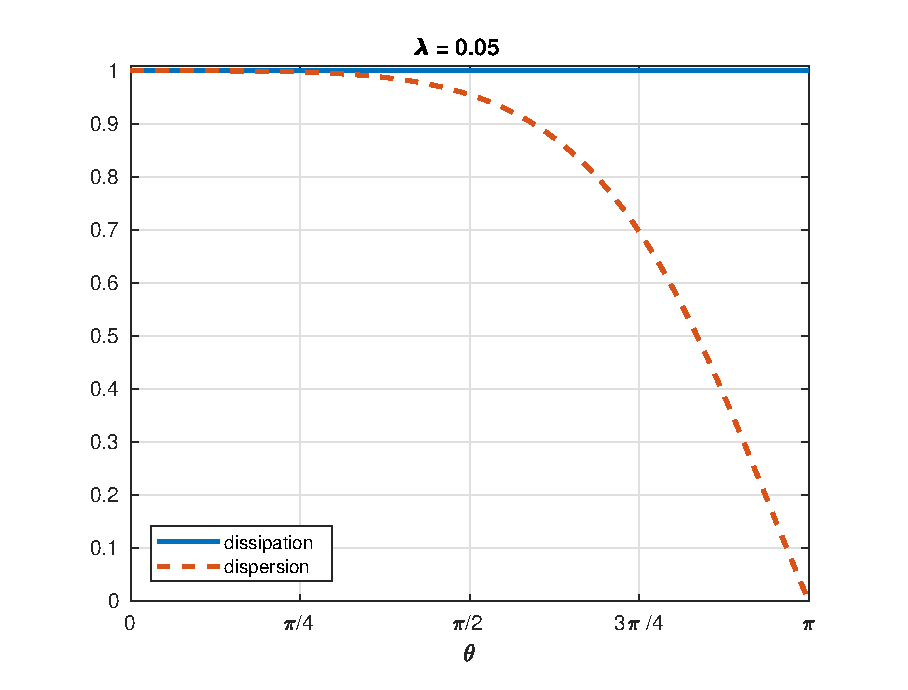
\includegraphics[scale=0.5]{dissip1.eps}
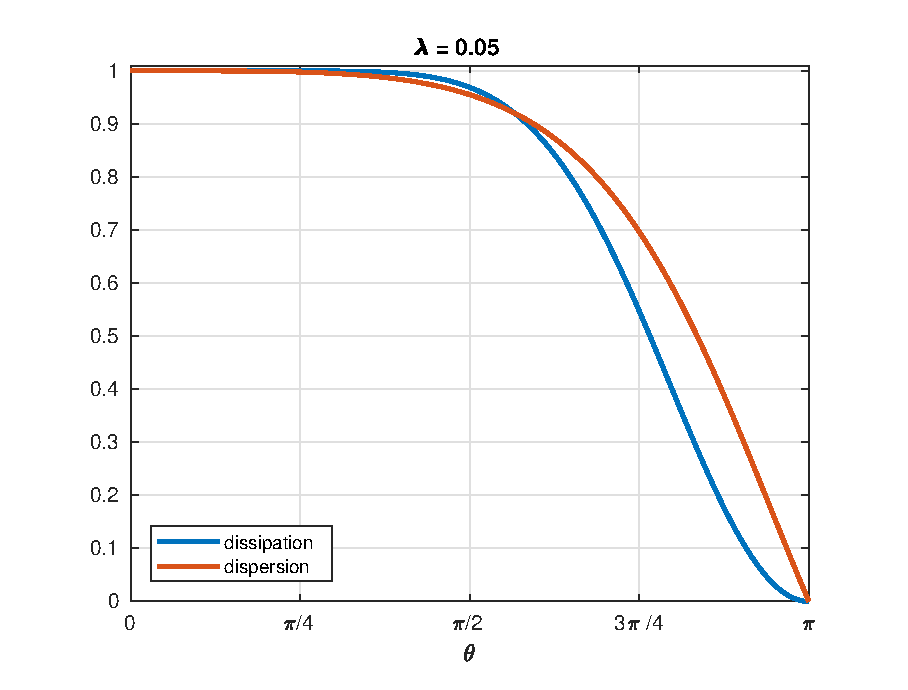
\includegraphics[scale=0.5]{dissipf1.eps}\\
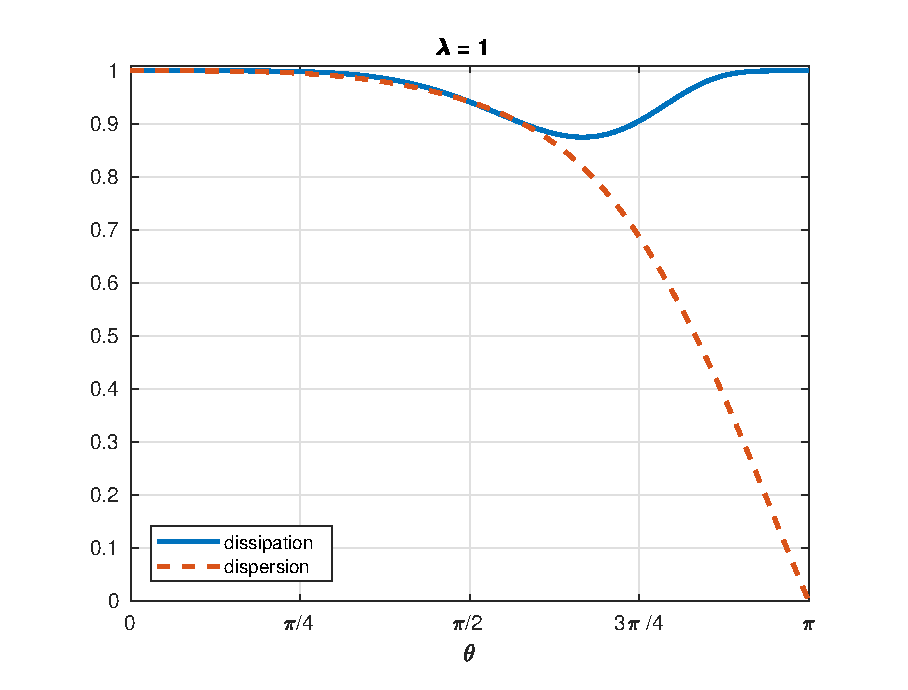
\includegraphics[scale=0.5]{dissip2.eps}
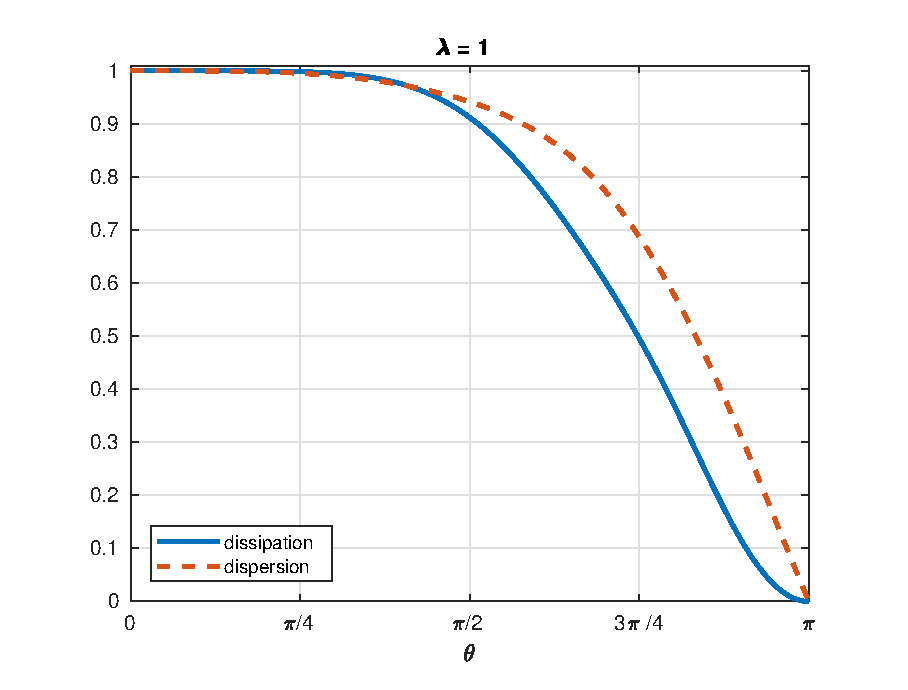
\includegraphics[scale=0.5]{dissipf2.eps}\\
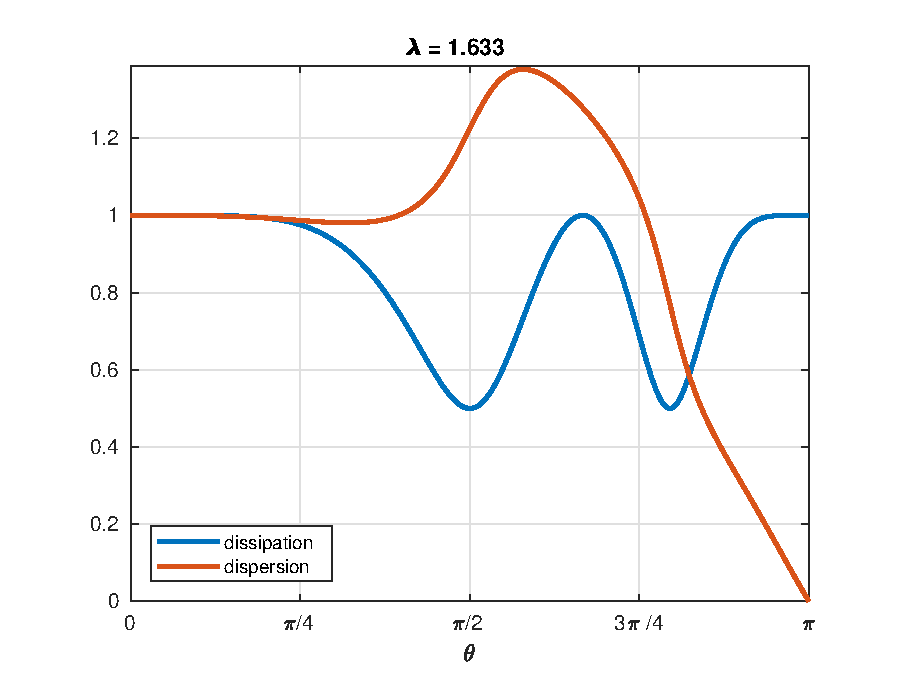
\includegraphics[scale=0.5]{dissip3.eps}
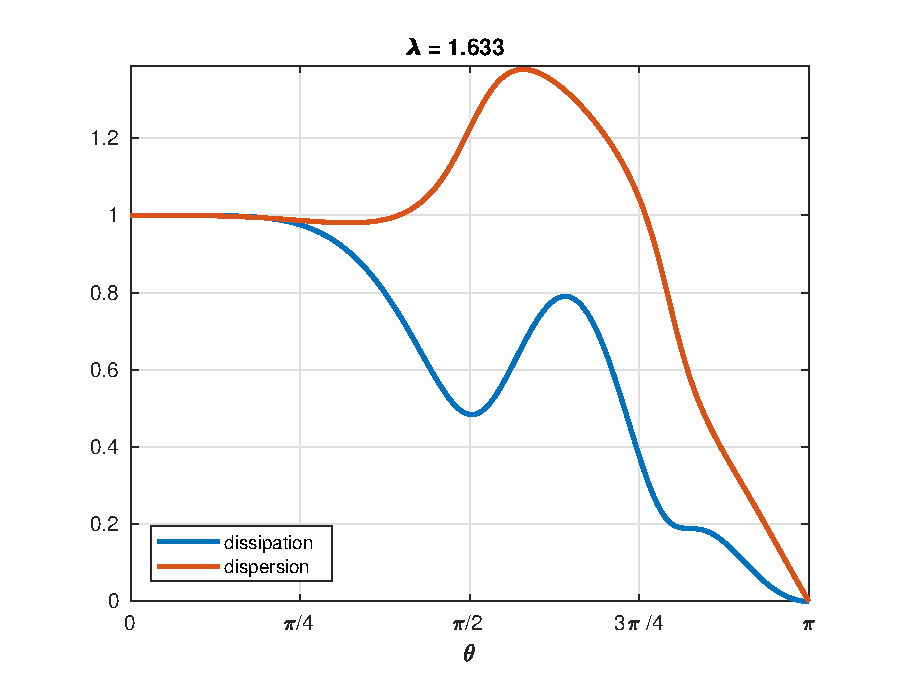
\includegraphics[scale=0.5]{dissipf3.eps}\\
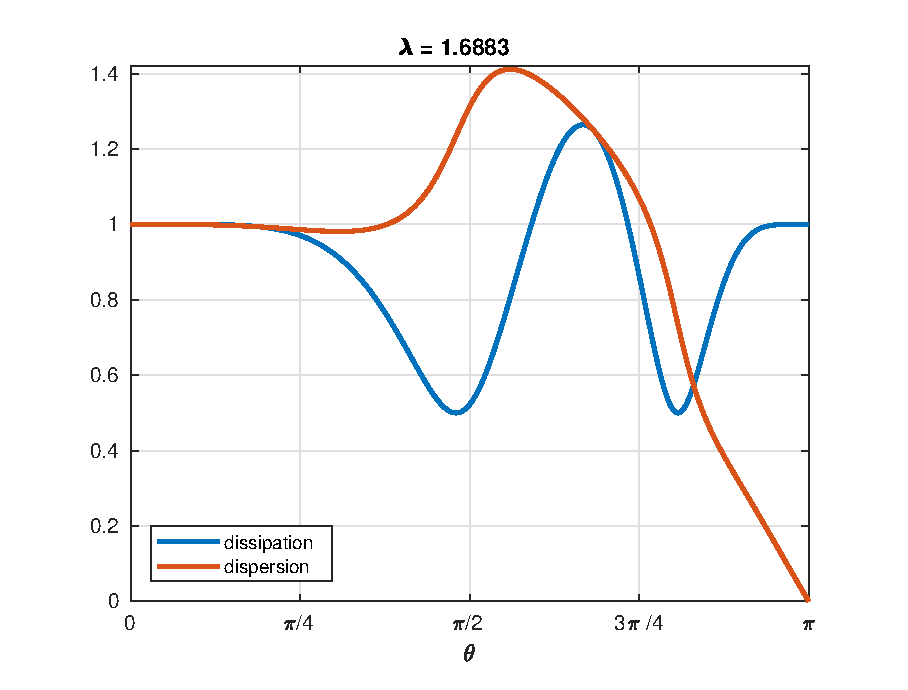
\includegraphics[scale=0.5]{dissip4.eps}
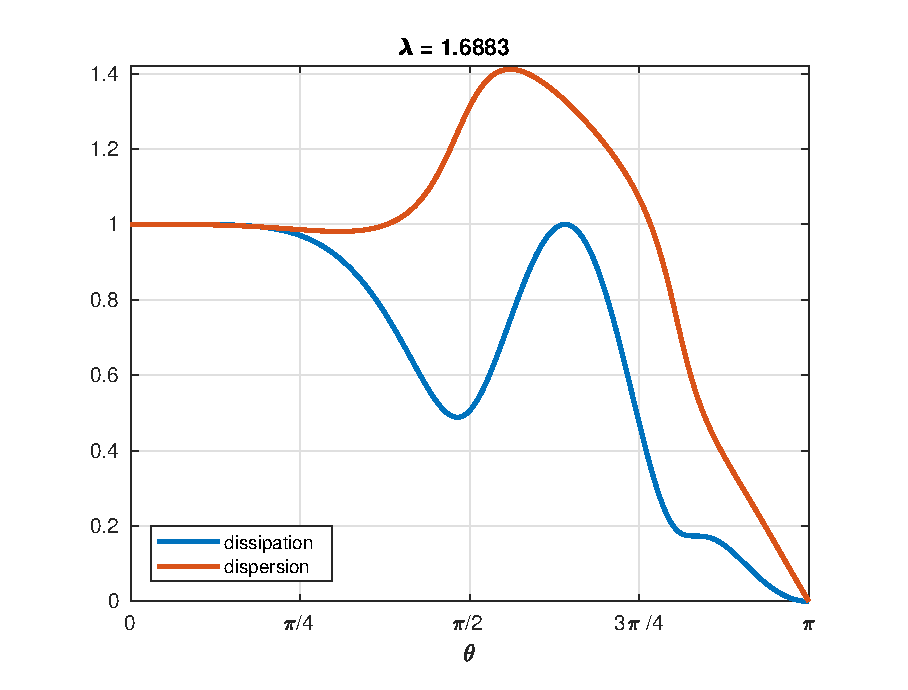
\includegraphics[scale=0.5]{dissipf4.eps}
\end{center}
\caption{Fonctions de dissipation et de dispersion associées à l'algorithme \ref{alg:RK4_transport1d} de résolution de l'équation \eqref{eq:transport_1D} sans un filtre (gauche) et avec filtre d'ordre 10 (droite) pour différentes valeurs de $\lambda = c \Delta t / h$.}
\label{fig:dissip_disper}
\end{figure}

Dans la figure \ref{fig:dissip_disper}, on représente la fonction de dissipation $\varepsilon_D$ et la fonction de dissipation $\varepsilon_{\Phi}$ pour différentes valeurs de $\lambda$. Le but est de comparer l'influence de l'opérateur de filtrage par rapport à l'absence d'opérateur de filtrage quand on utilise RK4 avec le schéma compact d'ordre 4 $\delta_{4,x}^H$.

A $\lambda$ fixé, on ne trace ces $\varepsilon_D$ et $\varepsilon_{\Phi}$ que pour $\theta \in [0, \pi]$ pour des raisons de parité. Lorsque $\lambda=0.05$, le schéma sans filtre est peu dissipatif. Le pas de temps $\Delta t$ est petit donc il y a peu d'action du schéma $RK4$. Le schéma est dispersif. En revanche, l'introduction du filtrage d'ordre 10 rend le schéma dissipatif. Lorsque $\lambda =1$, l'action de RK4 est plus importante le schéma est un peu plus dissipatif lorsque le filtrage est absent.
Le choix $\lambda = \lambda_{\infty}$, on se place à la limite de stabilité du schéma sans filtre. Dans ce cadre, deux zones pour lesquelles le schéma est dissipatif aparaissent. Lorsque l'on utilise le filtre d'ordre 10, le schéma est plus dissipatif, en particulier autour de $5 \pi/8$.
Lorsque $\lambda = 1.6883$, le schéma sans filtrage est instable. En revanche le schéma avec filtrage d'ordre 10 est à la limite de la stabilité. Il présente une bonne amplification et les ondes sont amorties lorsque $\theta \geq \pi/4$.







\subsection{Relations de conservations}

L'équation de transport \eqref{eq:transport_1D} est une équation de conservation. En effet il est immédiat que la périodicité de $x \mapsto u(t,x)$ entraine

\begin{proposition}
Si $u$ est une solution périodique de \eqref{eq:transport_1D} alors pour tout $t>0$, on a
\begin{equation}
\gint_0^1 u(t,x)dx = \gint_0^1 u_0(x)dx.
\end{equation}
\end{proposition}

Autrement dit, la masse totale de $u$ est conservée au cours du temps. Dans la pratique, la résolution par un schéma numérique peut entraîner une perte de conservation. 
La contrepartie discrète de la conservation de la masse est la proposition suivante :

\begin{proposition}
La suite $(\mathfrak{u}^n)$ est calculée par l'algorithme \ref{alg:RK4_transport1d} satisfait
\begin{equation}
(\mathfrak{u}^{n+1}, \mathfrak{1})_{h,\per} = (\mathfrak{u}^n, \mathfrak{1})_{h,\per}.
\end{equation}
pour tout $n \in \mathbb{N}$, avec $\mathfrak{1}$ est la fonction de grille constante égale à 1.
\end{proposition}

\begin{proof}
Soit $\mathfrak{b} \in l^2_{h,\per}$ une fonction de grille quelconque et $b=\vec(\mathfrak{b}) \in \mathbb{R}^N$, on a
\begin{align*}
(\delta_{4,x}^H \mathfrak{b}, \mathfrak{1})_{h,\per} & = \left( Q_4^H(T) b \right)^T \cdot \mathbf{1} \\
	& = \dfrac{1}{h} b^T \cdot (\bar{Q}_4^H(T) \mathbf{1}) \\
	& = \dfrac{1}{h} b^T \cdot \mathbf{0} \text{ par antisymétrie de }Q_4^H(T)\\
	& = 0.
\end{align*}
De cette égalité, on déduit
\begin{equation}
(K^{(i)}, \mathfrak{1})_{h,\per} = 0
\end{equation}
pour tout $i \in \left\lbrace 1, 2, 3, 4 \right\rbrace$ dans l'algorithme \ref{alg:RK4_transport1d}.

De là, on déduit :
\begin{align*}
(\mathfrak{u}^{n+1},\mathfrak{1})_{h,\per} & = h \left( S_{2J}(T) \left( U^n + \dfrac{\Delta t}{6}(K^{(1)}+2K^{(2)}+2K^{(3)}+K^{(4)})  \right) \right)^T \cdot \mathbf{1} \\
	& = h \left( U^n + \dfrac{\Delta t}{6}(K^{(1)}+2K^{(2)}+2K^{(3)}+K^{(4)})  \right)^T \cdot \mathbf{1} \text{ par symétrie de } S_{2J}(T)\\
	& = (\mathfrak{u}^n , \mathfrak{1})_{h,\per}.
\end{align*}
avec $U^n = \vec(\mathfrak{u}^n)$.
\end{proof}

\subsection{Résultats numériques}

Dans cette section, on évalue numériquement les performances du schéma numérique dans les deux cas suivants.

\subsubsection{Condition initiale régulière}

On considère la condition initiale $u_0$ donnée par 
\begin{equation}
u_0(x) = \dfrac{1}{\sqrt{2}} \left[ \cos (2 \pi x) \sin (4 \pi x) + \sin ( 2 \pi x ) \right] \text{ avec } x \in \Omega = [0,1],
\label{eq:transport1d_test_reg}
\end{equation}
avec $c=0.2$. On compare la solution exacte avec la solution numérique associée. L'erreur relative
\begin{equation}
e_l^n = \dfrac{\| \mathfrak{u}^n - u^*(t^n) \|_l}{\| u^*(t^n) \|_l}
\end{equation}
calculée au temps $t^n$. Les valeurs obtenues sont données dans la table \ref{tab:rate_transport1d_test_reg}. Les résultats permettent de confirmer la convergence à l'ordre 4 attendue.
\begin{table}[htbp]
\begin{center}
\begin{tabular}{|c||c|c|c|}
\hline
\textbf{N}  & \textbf{norme 2} & \textbf{norme $\infty$} \\
\hline
\hline
$50$   & $1.1158(-2)$  & $1.2630(-2)$  \\
$100$  & $7.1441(-4)$  & $8.0641(-4)$  \\
$500$  & $1.1484(-6)$  & $1.2998(-6)$  \\
$1000$ & $7.1839(-8)$  & $8.1303(-8)$  \\
\hline 
\hline
\textbf{ordre estimé}& $3.9917$ & $3.9913$\\
\hline
\end{tabular}
\end{center}
\caption{Equation de convection avec la condition initiale \eqref{eq:transport1d_test_reg}. Table de convergence de l'algorithme \ref{alg:RK4_transport1d} avec le filtre d'ordre 10. Le temps final est $T=10$ et $c \Delta t/h=1.5$.}
\label{tab:rate_transport1d_test_reg}
\end{table} 
L'erreur est tracée au cours du temps dans la figure \ref{fig:transport1d_test_reg} en $\| \cdot \|_2$ et $\| \cdot \|_{\infty}$.
\begin{figure}[htbp]
\begin{center}
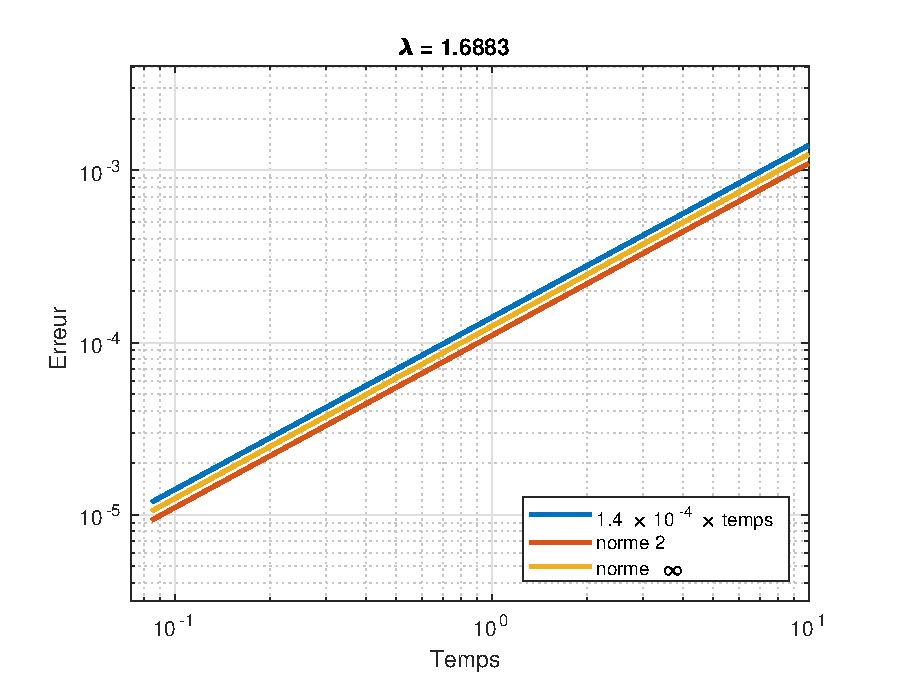
\includegraphics[scale=0.7]{erreurf2_reg.eps}
\end{center}
\caption{Equation de convection avec la condition initiale \eqref{eq:transport1d_test_reg}. Historique de l'erreur de l'algorithme \ref{alg:RK4_transport1d} avec le filtre d'ordre 10 et la condition initiale \eqref{eq:transport1d_test_reg}. On choisit $N=100$ points de grille et $c \Delta t/h = 1.6883$ ($118$ itérations).}
\label{fig:transport1d_test_reg}
\end{figure}
Comme donné dans la proposition \ref{prop:consistance_h_trsp}, on observe la dépendance linéaire en $t$ de l'erreur.








\subsubsection{Condition initiale de type créneau}

On considère à présent la donnée initiale
\begin{equation}
u_0(x) = \left\lbrace
\begin{array}{rl}
1 & \text{ si } 0.25 \leq x \leq 0.75, \\
-1 & \text{sinon,}
\end{array}
\right.
\text{ pour } x \in \Omega = [0,1],
\label{eq:transport1d_test_irreg}
\end{equation}
avec $c=0.2$. Les résultats numériques pour la convection de la donnée initiale \eqref{eq:transport1d_test_irreg} sont donnés dans la figure \ref{fig:comp_ireg} au temps final $t=10$, c'est à dire au bout de deux périodes.

Des oscillations parasites de nature dispersive apparaissent. Ces oscillations peuvent être atténuées par l'utilisation d'un filtre. On compare sur la figure \ref{fig:comp_ireg} la solution au temps $t=10$ avec les solution obtenues en utilisant différentes fonctions de filtrage dans l'algorithme \ref{alg:RK4_transport1d}.

On constate que le filtre d'ordre 2 permet de supprimer les ondes parasites mais est trop dissipatif. Les filtres d'ordres 4, 6, 8 et 10 donnent des résultats moins dissipatif tout en atténuant les oscillations dispersives.

\begin{figure}[htbp]
\begin{center}
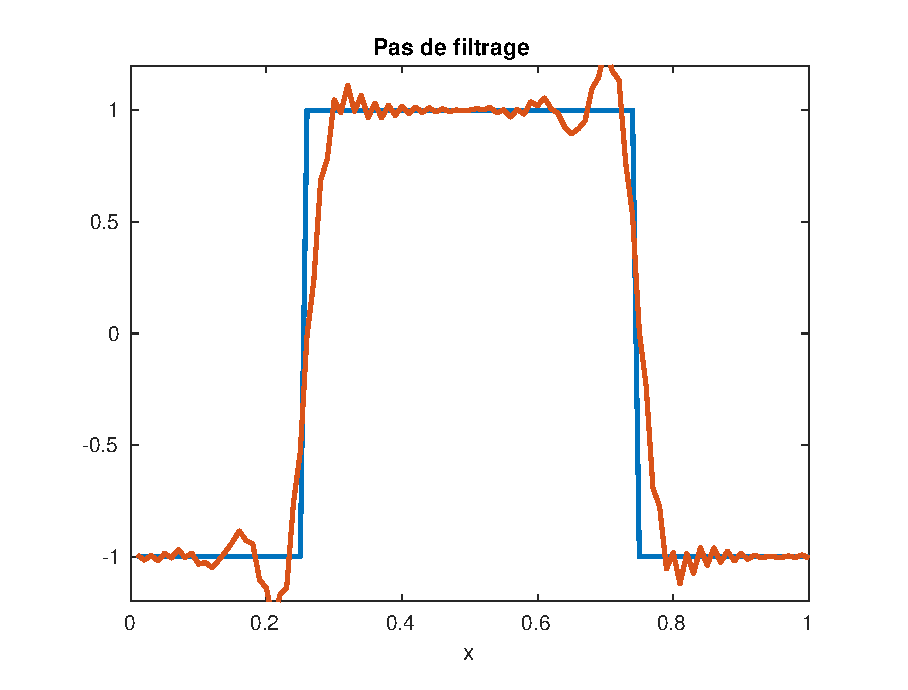
\includegraphics[scale=0.5]{creneau_noftr.eps}
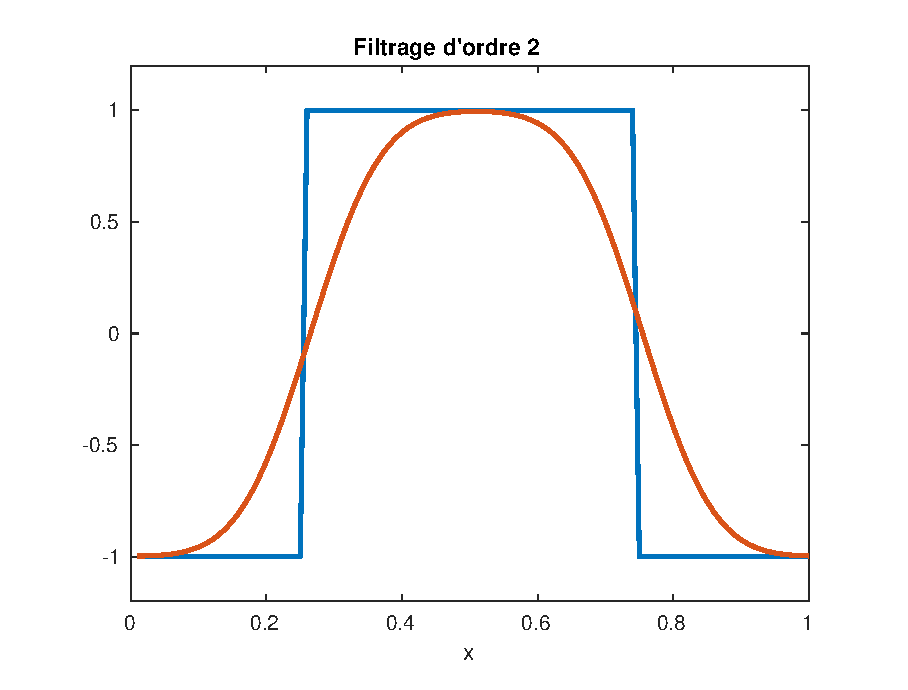
\includegraphics[scale=0.5]{creneau_ftr2.eps}\\
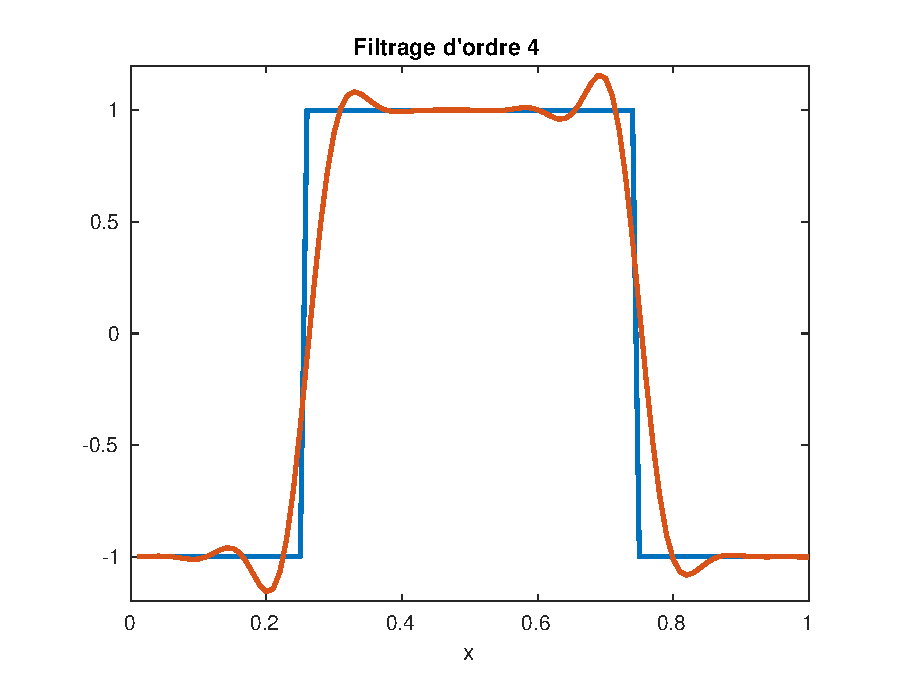
\includegraphics[scale=0.5]{creneau_ftr4.eps}
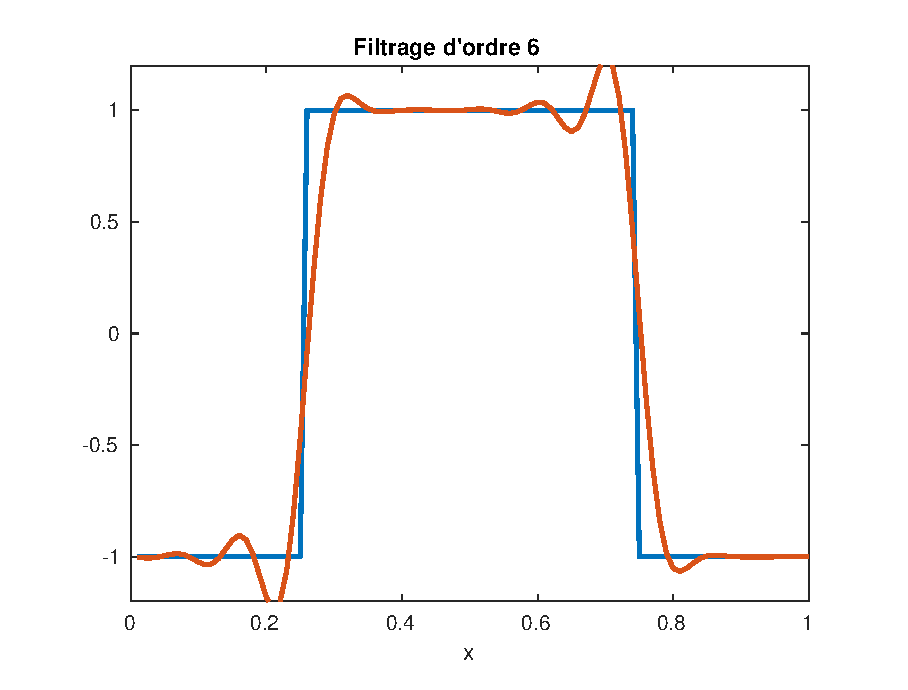
\includegraphics[scale=0.5]{creneau_ftr6.eps}\\
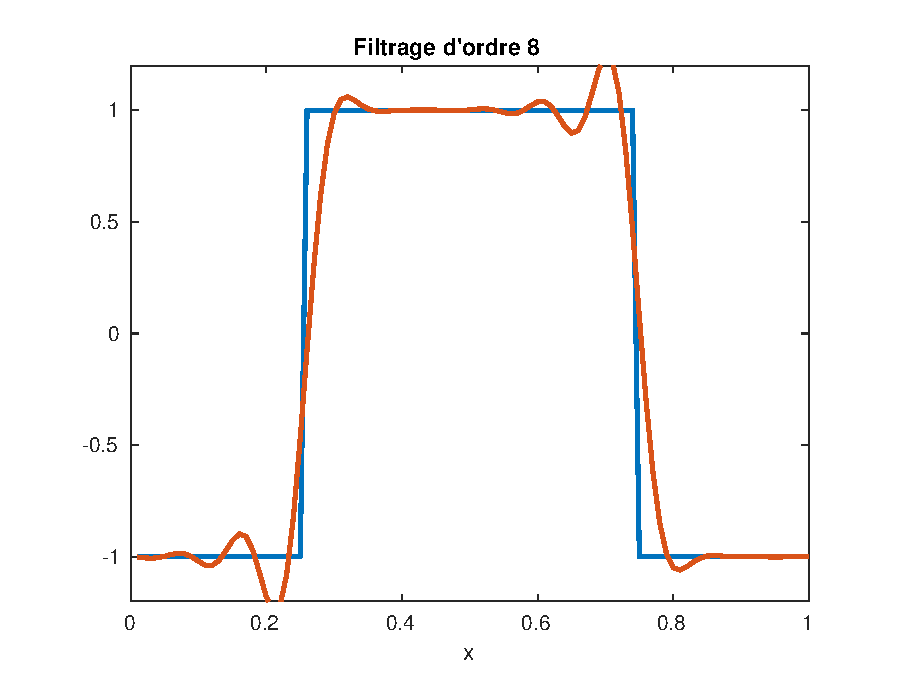
\includegraphics[scale=0.5]{creneau_ftr8.eps}
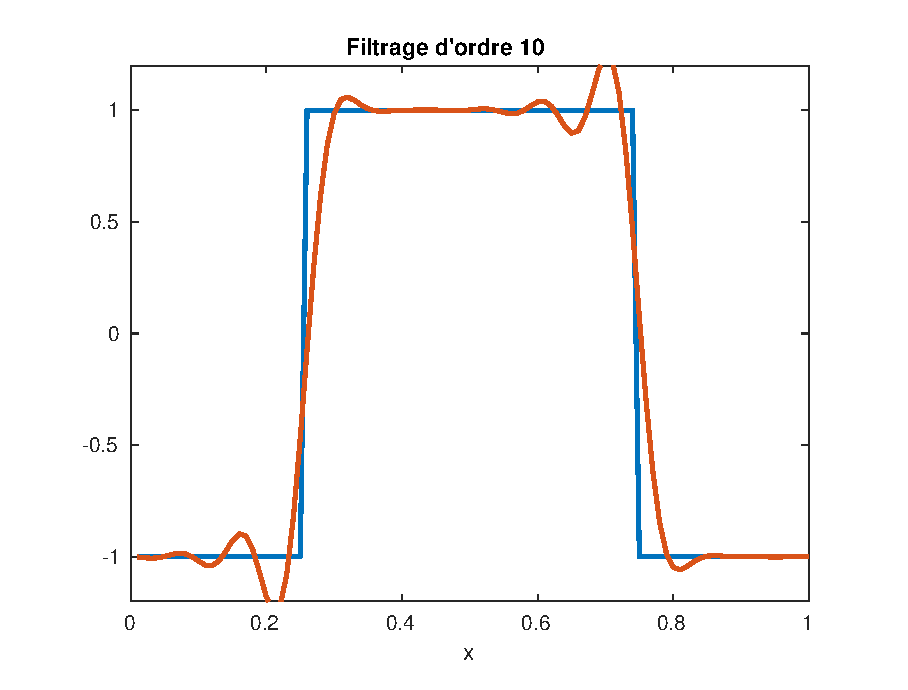
\includegraphics[scale=0.5]{creneau_ftr10.eps}\\
\end{center}
\caption{Comparaison de la solution exacte (bleu) avec la solution obtenue par l'algorithme \ref{alg:RK4_transport1d} (rouge) au temps $t=10$ pour la résolution de l'équation \eqref{eq:transport_1D} avec différents filtres. $\lambda = c \Delta t / h = 1.5$ et $N=100$. Les résultats sont obtenus en $133$ itérations et au bout de 2 périodes.}
\label{fig:comp_ireg}
\end{figure}

Il est bien connu que l'ammélioration du comportement dissipatif d'un schéma centré de type \eqref{eq:transport_1D_SD} est un problème délicat. On renvoie à ce sujet aux méthodes d'hyperviscosités \cite{Cook2005}, aux méthodes non linéaires de type WENO \cite{Qiu2002} ou aux méthodes utilisant des senseurs non linéaires \cite{Yee1989}. Nous n'allons pas plus loin dans cette direction car les expériences numériques effectuées pour des problèmes sphériques en climatologie numérique n'ont pas nécessités de tels traitements.














































\section{Équation des ondes en dimension 2}

On considère dans cette partie l'équation des ondes sur un carré périodique avec un paramètre $f > 0$ représentant la force de Coriolis. Cette équation peut être comme la linéarisation de l'équation Shallow Water  au voisinage d'un état de repos.

Pour $(x,y) \in \Omega = [0,1]^2$ et $t>0$, elle s'écrit 
\begin{equation}
\left\lbrace
\begin{array}{rcl}
\dfrac{\partial \eta}{\partial t} + H \left( \dfrac{\partial u}{\partial x} + \dfrac{\partial v}{\partial y} \right) & = & 0 \\
\dfrac{\partial u}{\partial t} + g \dfrac{\partial \eta}{\partial x} - f v & = & 0 \\
\dfrac{\partial v}{\partial t} + g \dfrac{\partial \eta}{\partial y} + f u & = & 0 \\
\end{array}
\right.
\label{eq:ondes_2D}
\end{equation}
La constante $H>0$ est une hauteur de fluide de référence et $g>0$ est la constante de gravité.
On ajoute, à cette équation, une condition initiale $1-$périodique de la forme
\begin{equation}
\left\lbrace
\begin{array}{rcl}
\eta(0,x,y) & = & \eta_0(x,y)\\
u(0,x,y) & = & u_0(x,y)\\
v(0,x,y) & = & v_0(x,y)
\end{array}
\right. \text{ avec } (x,y) \in \Omega. 
\end{equation}


\begin{proposition}
Si $\eta(t,x,y)$, $u(t,x,y)$ et $v(t,x,y)$ sont trois fonctions de $\mathbb{R}^+ \times \omega$ dans $\mathbb{R}$ solutions de \eqref{eq:ondes_2D}. Alors les relations de conservation suivantes sont vérifiées :
\begin{itemize}
\item \textbf{Conservation de la masse :}
\begin{equation}
\dfrac{d}{dt} \gint_{\Omega} h(t,x,y)dxdy = 0,
\end{equation}
\item \textbf{Conservation de l'énergie :}
\begin{equation}
\dfrac{d}{dt} \gint_{\Omega} \left( \dfrac{1}{2} g h(t,x,y)^2 + \dfrac{1}{2} H \left( u(t,x,y)^2 + v(t,x,y)^2 \right) \right) dxdy = 0.
\end{equation}
\end{itemize}
\end{proposition}

\begin{proof}
Soient $\eta$, $u$ et $v$ trois fonctions de $\mathbb{R}^+ \times [0,1]^2$ dans $\mathbb{R}$ solutions de \eqref{eq:ondes_2D} alors :
\begin{itemize}
\item \textbf{Conservation de la masse :}
\begin{align*}
\dfrac{d}{dt} \gint_{[0,1]^2} \eta(t,x,y)dxdy & = - H \gint_{[0,1]^2} \dfrac{\partial u}{\partial x}(t,x,y) + \dfrac{\partial v}{\partial y}(t,x,y) dx dy \\
	& - H \gint_0^1 \left( u(t,1,y) - u(t,0,y) \right)dy  - H \gint_0^1 \left( u(t,x,1) - u(t,x,0) \right)dx \\
	& = 0 \text{ par périodicité de } u \text{ et } v. 
\end{align*}

\item \textbf{Conservation de l'énergie :} en multipliant la première équation de \eqref{eq:ondes_2D} par $\eta$ et en intégrant, on a 
\begin{align*}
\dfrac{1}{2} \dfrac{d}{dt} \gint_{[0,1]^2} \eta(t,x,y)^2 dx dy & = \gint_{[0,1]^2} \eta(t,x,y) \dfrac{\partial \eta}{\partial t}(t,x,y) dx dy \\
	& = - H \gint_{[0,1]^2} \eta(t,x,y) \left( \dfrac{\partial u}{\partial x}(t,x,y) + \dfrac{\partial v}{\partial y}(t,x,y) \right) dx dy.
\end{align*}
D'autres part, on a 
\begin{align*}
\dfrac{1}{2} \dfrac{d}{dt} \gint_{[0,1]^2} u(t,x,y)^2 dx dy & = \gint_{[0,1]^2} u(t,x,y) \dfrac{\partial u}{\partial t}(t,x,y) dx dy \\
& = \gint_{[0,1]^2} f u(t,x,y) v(t,x,y) - g u(t,x,y) \dfrac{\partial \eta}{\partial x}(t,x,y) dx dy,
\end{align*}
ainsi que 
\begin{equation*}
\dfrac{1}{2} \dfrac{d}{dt} \gint_{[0,1]^2} v(t,x,y)^2 dx dy =  \gint_{[0,1]^2}  - f u(t,x,y) v(t,x,y) - g u(t,x,y) \dfrac{\partial \eta}{\partial y}(t,x,y) dx dy.
\end{equation*}
En combinant ces trois dernières relations, on obtient
\begin{multline*}
\dfrac{d}{dt} \gint_{[0,1]^2} \left( \dfrac{1}{2} g h(t,x,y)^2 + \dfrac{1}{2} H \left( u(t,x,y)^2 + v(t,x,y)^2 \right) \right) = \\
- g H \gint_{[0,1]^2} \dfrac{\partial}{\partial x} \left( \eta(t,x,y) u (t,x,y) \right) +  \dfrac{\partial}{\partial y} \left( \eta(t,x,y) v (t,x,y) \right) dx dy
= 0
\end{multline*}
en utilisant la périodicité de $\eta$, $u$ et $v$.
\end{itemize}
\end{proof}







\subsection{Schéma centré en dimension 2}

De façon analogue à l'équation de transport \eqref{eq:transport_1D}, on utilise la méthode des lignes. La version demidiscrétisée de \eqref{eq:ondes_2D} est
\begin{equation}
\left\lbrace
\begin{array}{rcl}
\dfrac{d \etafrak}{dt} + H ( \delta_{x,4}^H \mathfrak{u} + \delta_{y,4}^H \mathfrak{v} ) & = & 0 \\
\dfrac{d \mathfrak{u}}{dt} + g \delta_{x,4}^H \etafrak - f \mathfrak{v} & = & 0 \\
\dfrac{d \mathfrak{v}}{dt} + g \delta_{y,4}^H \etafrak + f \mathfrak{u} & = & 0. \\
\end{array}
\right.
\label{eq:ondes_2D_SD}
\end{equation}
On cherche alors $t \mapsto \etafrak(t) \in L^2_{h,\per}$, $t \mapsto \mathfrak{u}(t) \in L^2_{h,\per}$ et $t \mapsto \mathfrak{v}(t) \in L^2_{h,\per}$ des approximations de $\eta$, $u$ et $v$ les solutions de \eqref{eq:ondes_2D} aux points du maillage.

Ce sont effectivement des approximations comme le montre la proposition suivante :

\begin{proposition}
$\etafrak$, $\mathfrak{u}$ et $\mathfrak{v}$ solutions de \eqref{eq:ondes_2D_SD} convergent vers $\eta$, $u$ et $v$ solutions de \eqref{eq:ondes_2D} sur $[0,T]$ au sens où il existe $\tilde{C}>0$ indépendant de $t$, $\etafrak$, $u$ et $v$ tel que
\begin{equation}
E(t) \leq g H t C h^4
\end{equation}
avec $C = \tilde{C} \max_{t \in [0,T]} \left( \dfrac{1}{\sqrt{H}} \| \partial_x^{(5)} u \|_{\infty}, \dfrac{1}{\sqrt{H}} \| \partial_y^{(5)} v \|_{\infty}, \dfrac{1}{\sqrt{g}} \| \partial_x^{(5)} \eta \|_{\infty}, \dfrac{1}{\sqrt{g}} \| \partial_y^{(5)} \eta \|_{\infty}  \right)$
et en notant les termes d'erreur $\mathfrak{e}_{\eta} = \eta^* - \etafrak$, $\mathfrak{e}_{u} = u^* - \mathfrak{u}$ et $\mathfrak{e}_{v} = v^* - \mathfrak{v}$ ainsi que $E(t) = \sqrt{ g \| \mathfrak{e}_{\eta} \|^2_{h,\per} + H \| \mathfrak{e}_u \|^2_{h,\per} + H \| \mathfrak{e}_v \|^2_{h,\per}}$.
\end{proposition}


















































\begin{proof}
On définit les termes de troncature $\mathbf{\tau}_x \eta = \delta_{4,x}^H \etafrak- (\partial_x \eta)^*$, $\mathbf{\tau}_y \eta = \delta_{4,y}^H \etafrak- (\partial_y \eta)^*$, $\mathbf{\tau}_x u = \delta_{4,x}^H \mathfrak{u}- (\partial_x u)^*$ et $\mathbf{\tau}_y v = \delta_{4,y}^H \mathfrak{v}- (\partial_y v)^*$.

Les termes d'erreurs sont solutions de 
\begin{equation}
\left\lbrace
\begin{array}{rcccl}
\dfrac{d}{dt} \mathfrak{e}_{\eta} & = &  H \left( \delta_{4,x}^H \mathfrak{e}_u + \delta_{4,y}^H \mathfrak{e}_v \right) & + & H \left( \tau_x u + \tau_y v \right)\\
\dfrac{d}{dt} \mathfrak{e}_u & = & -g \delta_{4,x}^H \mathfrak{e}_{\eta} + f \mathfrak{e}_v & - & g \tau_x \eta \\
\dfrac{d}{dt}\mathfrak{e}_v & = & - g \delta_{4,y}^H \mathfrak{e}_{\eta} - f \mathfrak{e}_u
 & - & g \tau_y \eta  \end{array}
\right.
\end{equation}

Par produit scalaire avec $\mathfrak{e}_{\eta}$ de la première équation on obtient :
\begin{equation}
\dfrac{1}{2} \dfrac{d}{dt} \| \mathfrak{e}_{\eta} \|_{h,\per}^2 = (\dfrac{d}{dt} \mathfrak{e}_{\eta}, \mathfrak{e}_{\eta})_{h,\per} = - H ( \delta_{4,x}^H \mathfrak{e}_{u} + \delta_{4,y}^H \mathfrak{e}_{v}, \mathfrak{e}_{\eta})_{h,\per}  + H ( \tau_x u + \tau_y v, \mathfrak{e}_{\eta})_{h,\per}
\label{eq:consist_ondes1}
\end{equation}
En effectuant les produits scalaires de la seconde et troisième équation par $\mathfrak{e}_u$ et $\mathfrak{e}_v$, on obtient :
\begin{equation}
(\dfrac{d}{dt} \mathfrak{e}_u, \mathfrak{e}_u)_{h,\per} = - g (\delta_{4,x}^H \mathfrak{e}_{\eta}, \mathfrak{e}_u)_{h,\per} + f(\mathfrak{e}_v, \mathfrak{e}_u)_{h,\per} - g(\tau_x \eta, \mathfrak{e}_u)_{h,\per}
\end{equation}
ainsi que 
\begin{equation}
(\dfrac{d}{dt} \mathfrak{e}_v, \mathfrak{e}_v)_{h,\per} = - g (\delta_{4,y}^H \mathfrak{e}_{\eta}, \mathfrak{e}_v)_{h,\per} - f(\mathfrak{e}_u, \mathfrak{e}_v)_{h,\per} - g(\tau_y \eta, \mathfrak{e}_v)_{h,\per}.
\end{equation}
Alors, en sommant ces deux équations et, par antisymétrie de $\delta_{4,x}^H$ et de $\delta_{4,y}^H$, on a
\begin{equation}
\dfrac{1}{2} \dfrac{d}{dt} \left( \| \mathfrak{e}_{u} \|_{h,\per}^2 + \| \mathfrak{e}_{v} \|_{h,\per}^2 \right) = (d_t \mathfrak{e}_u, \mathfrak{e}_u)_{h,\per}) + (d_t \mathfrak{e}_v, \mathfrak{e}_v)_{h,\per} 
\end{equation}
d'où 
\begin{equation}
\dfrac{1}{2} \dfrac{d}{dt} \left( \| \mathfrak{e}_{u} \|_{h,\per}^2 + \| \mathfrak{e}_{v} \|_{h,\per}^2 \right) = g (\delta_{4,x}^H \mathfrak{e}_u + \delta_{4,y}^H \mathfrak{e}_v, \mathfrak{e}_{\eta})_{h,\per} - g(\tau_x \eta, \mathfrak{e}_u)_{h,\per} - g(\tau_y \eta, \mathfrak{e}_v)_{h,\per}.
\label{eq:consist_ondes2}
\end{equation}
En sommant $g \times $\eqref{eq:consist_ondes1} $+ H \times$\eqref{eq:consist_ondes2}, on obtient :
\begin{equation}
\dfrac{d}{dt} E^2(t) = 2 g H \left( (\tau_x u + \tau_y v, \mathfrak{e}_{\eta})_{h,\per} - (\tau_x \eta, \mathfrak{e}_u )_{h,\per} - (\tau_y \eta, \mathfrak{e}_v )_{h,\per} \right).
\end{equation}
En majorant le terme de droite par sa valeur absolue, on obtient
\begin{equation}
\dfrac{d}{dt} E^2(t) \leq 2 g H \left( |(\tau_x u + \tau_y v, \mathfrak{e}_{\eta})_{h,\per}| + |(\tau_x \eta, \mathfrak{e}_u )_{h,\per}| + |(\tau_y \eta, \mathfrak{e}_v )_{h,\per}|  \right).
\end{equation}
Alors, pour tout $\alpha >0$, on a
\begin{equation}
\dfrac{d}{dt}E^2(t) \leq 2 gH \left( \dfrac{\alpha}{H} \| \tau_x u + \tau_y v \|_{h,\per}^2 + \dfrac{H}{\alpha} \| \mathfrak{e}_{\eta} \|_{h,\per}^2 + \dfrac{\alpha}{g} \| \tau_x \eta \|_{h,\per}^2 + \dfrac{\alpha}{g} \| \tau_y \eta \|_{h,\per}^2  + \dfrac{g}{\alpha} \| \mathfrak{e}_u \|_{h,\per}^2 + \dfrac{g}{\alpha} \| \mathfrak{e}_v \|_{h,\per}^2  \right).
\end{equation}
Ainsi, si on pose 
\begin{equation}
\Upsilon(t) = \dfrac{1}{H} \| \tau_x u + \tau_y v \|_{h,\per} + \dfrac{1}{g} \| \tau_x \eta \|_{h,\per}^2 + \dfrac{1}{g} \| \tau_y \eta \|_{h,\per}^2
\end{equation}
on obtient
\begin{equation}
\dfrac{d}{dt}E^2(t) \leq 2gh \left( \alpha \Upsilon(t) + \dfrac{1}{g} E^2(t) \right).
\end{equation}
Par consistance des opérateurs $\delta_{4,x}^H$ avec $\partial_x$ et $\delta_{4,y}^H$ avec $\partial_y$, il existe $C_1>0$ indépendant des fonctions $\eta$, $u$ $v$ et $h$ tels que pour tout $t \in [0,T]$
\begin{equation}
\Upsilon(t) \leq C_1 h^8 \max_{t \in [0,T]} \left( \dfrac{1}{\sqrt{H}} \| \partial_x^{(5)} u \|_{\infty}, \dfrac{1}{\sqrt{H}} \| \partial_y^{(5)} v \|_{\infty}, \dfrac{1}{\sqrt{g}} \| \partial_x^{(5)} \eta \|_{\infty}, \dfrac{1}{\sqrt{g}} \| \partial_y^{(5)} \eta \|_{\infty}  \right) = h^8 \Upsilon_{\infty}.
\end{equation}
Ainsi, on a
\begin{equation}
\dfrac{d}{dt}E^2(t) \leq 2gh \left( \alpha h^8 \Upsilon_{\infty} + \dfrac{1}{\alpha} E^2(t) \right),
\label{eq:proof_cons_lswe}
\end{equation}
et d'après le lemme Gronwall,
\begin{equation}
E^2(t) \leq \alpha^2 h^8 \Upsilon_{\infty} \left( \exp \left( \dfrac{2gHt}{\alpha}  \right) -1 \right).
\end{equation}
Pour tout $t>0$ fixé, on pose $\beta = \alpha /(2gHt)$, l'équation \eqref{eq:proof_cons_lswe} se réécrit
\begin{equation}
E^2(t) \leq 4 g^2 H^2 t^2 h^8 \Upsilon_{\infty} a(\beta)
\end{equation}
avec $a$ la fonction donnée par
\begin{equation}
a : \beta > 0 \mapsto \beta^2 \left( \exp \left(\dfrac{1}{\beta} \right) -1 \right).
\end{equation}
Or, la fonction $a(\beta)$ est continue, positive et
\begin{equation}
\lim_{\beta \rightarrow + \infty} a(\beta) = \lim_{\beta \rightarrow 0} a(\beta) = + \infty.
\end{equation}
Donc il existe $m>0$ tel que pour tout $\beta>0$, on ait $a(\beta)>m$. On obtient $m \geq 1.545$. Ainsi, on a
\begin{equation}
E^2(t) \leq g^2 H^2 t^2 C_1 m \Upsilon_{\infty} h^8.
\end{equation}
On conclut en prenant la racine carrée de cette dernière relation.
\end{proof}

De plus, le système semi-discrétisé \eqref{eq:ondes_2D_SD}vérifie des relations de conservations très semblables à celles de l'équation d'origine \eqref{eq:ondes_2D}.

\begin{proposition}
Si $\etafrak$, $\mathfrak{u}$ et $\mathfrak{v}$ sont solutions de \eqref{eq:ondes_2D_SD} alors les relations de conservation suivantes sont vérifiées :
\begin{itemize}
\item \textbf{Conservation de la masse :}
\begin{equation}
\dfrac{d}{dt} (\etafrak, \mathfrak{1})_{h,\per} = 0.
\end{equation}
\item \textbf{Conservation de l'énergie :}
\begin{equation}
\dfrac{d}{dt} \left( \dfrac{1}{2} g \| \etafrak \|_{h,\per}^2 + \dfrac{1}{2} H ( \| \mathfrak{u} \|_{h,\per}^2 +  \| \mathfrak{v} \|_{h,\per}^2) \right) = 0.
\end{equation}
\end{itemize}
\end{proposition}

\begin{proof}
\begin{itemize}
\item \textbf{Conservation de la masse :}
par consistance des opérateurs $\delta_{4,x}^H$ et $\delta_{4,y}^H$ avec $\partial_x$ et $\partial_y$, on note que $\delta_{4,x}^H \mathfrak{1} = \mathfrak{0}$ et $\delta_{4,y}^H \mathfrak{1} = \mathfrak{0}$, où $\mathfrak{1}$ (resp. $\mathfrak{0}$) est la fonction de grille égale à $1$ (resp. $0$). De là, il découle :
\begin{align*}
\dfrac{d}{dt} (\etafrak, \mathfrak{1})_{h,\per} & = ( d_t \etafrak, \mathfrak{1} )_{h,\per} \\
	& = - H (\delta_{4,x} \mathfrak{u}, \mathfrak{1})_{h,\per} - H (\delta_{4,y} \mathfrak{v}, \mathfrak{1})_{h,\per} \\
	& = H (\mathfrak{u}, \delta_{4,x} \mathfrak{1})_{h,\per} + H (\mathfrak{v}, \delta_{4,y} \mathfrak{1})_{h,\per} \\
	& = 0
\end{align*}
où on a utilisé l'anti-symétrie des opérateurs.

\item \textbf{Conservation de l'énergie :}
On a
\begin{equation}
(\dfrac{d}{dt}\etafrak, \etafrak)_{h,\per} = \dfrac{1}{2} \dfrac{d}{dt} \| \etafrak \|^2_{h,\per} = - H (\delta_{4,x} \mathfrak{u}, \etafrak)_{h,\per} - H (\delta_{4,y} \mathfrak{v}, \etafrak)_{h,\per}.
\end{equation}
De même, on a :
\begin{equation}
\dfrac{1}{2} \dfrac{d}{dt} (\| \mathfrak{u} \|_{h,\per}^2 + \| \mathfrak{v} \|_{h,\per}^2) = g (\delta_{4,x}^H \mathfrak{u}+\delta_{4,y}^H \mathfrak{v}, \etafrak)_{h,\per}.
\end{equation}
Par combinaison, on obtient :
\begin{equation}
\dfrac{d}{dt} \left( \dfrac{1}{2} g \| \etafrak \|_{h,\per}^2 + \dfrac{1}{2} H ( \| \mathfrak{u} \|_{h,\per}^2 +  \| \mathfrak{v} \|_{h,\per}^2) \right) = 0.
\end{equation}
\end{itemize}
\end{proof}

A partir d'ici, on pose $F_h : (L_{h,\per}^2)^3 \rightarrow (L_{h,\per}^2)^3$ l'application linéaire définie par
\begin{equation}
F_h : \begin{pmatrix}
\etafrak \\ \mathfrak{u} \\ \mathfrak{v}
\end{pmatrix} \mapsto \begin{pmatrix}
- H (\delta_{4,x}^H \mathfrak{u} + \delta_{4,y}^H \mathfrak{v}) \\
- g \delta_{4,x}^H \etafrak + f \mathfrak{v} \\
- g \delta_{4,y}^H \etafrak - f \mathfrak{u}
\end{pmatrix}.
\end{equation}
alors, le problème \eqref{eq:ondes_2D_SD} s'écrit
\begin{equation}
\dfrac{d}{dt} \begin{pmatrix}
\etafrak \\ \mathfrak{u} \\ \mathfrak{v}
\end{pmatrix} = F_h\begin{pmatrix}
\etafrak \\ \mathfrak{u} \\ \mathfrak{v}
\end{pmatrix}.
\end{equation}
On note $\Delta t>0$ le pas de temps et $\etafrak^n$, $\mathfrak{u}^n$ et $\mathfrak{v}^n$ les approximations de $\etafrak(n\Delta t)$, $\mathfrak{u}(n \Delta t)$ et $\mathfrak{v}(n \Delta t)$ obtenues par un algorithme de type RK4 filtré. On note $\mathcal{F}_{2F} = \mathcal{F}_{2F,x} \circ \mathcal{F}_{2F,y}$ l'opérateur de filtrage tel que $\mathcal{F}_{2F,x}$ (resp. $\mathcal{F}_{2F,y}$) est un opérateur de filtrage dans la direction de $x$ (resp. $y$). La méthode est détaillé dans l'algorithme \ref{alg:RK4_ondes2d}.

\begin{center}
\begin{minipage}[H]{12cm}
  \begin{algorithm}[H]
    \caption{: Schémas en temps RK4 avec étape de filtrage pour le système périodique \eqref{eq:ondes_2D_SD}}\label{alg:RK4_ondes2d}
    \begin{algorithmic}[1]
    \State $\etafrak^0 = \eta_0^*$, $\mathfrak{u}^0 = u_0^*$ et $\mathfrak{v}^0 = v_0^*$ connus,
    \For{$n=0,1, \ldots$}
             \State  $\left(K^{(1)}_{\eta}, K^{(1)}_{u}, K^{(1)}_{v}\right) = F_h(\etafrak^n, \mathfrak{u}^n, \mathfrak{v}^n)$,
             \State  $\left(K^{(2)}_{\eta}, K^{(2)}_{u}, K^{(2)}_{v}\right) = F_h\left(\etafrak^n + \dfrac{\Delta t}{2}K^{(1)}_{\eta}, \mathfrak{u}^n + \dfrac{\Delta t}{2}K^{(1)}_{u}, \mathfrak{v}^n + \dfrac{\Delta t}{2}K^{(1)}_{v}\right)$,
             \State   $\left(K^{(3)}_{\eta}, K^{(3)}_{u}, K^{(3)}_{v}\right) = F_h\left(\etafrak^n + \dfrac{\Delta t}{2}K^{(2)}_{\eta}, \mathfrak{u}^n + \dfrac{\Delta t}{2}K^{(2)}_{u}, \mathfrak{v}^n + \dfrac{\Delta t}{2}K^{(2)}_{v}\right)$,
             \State   $\left(K^{(4)}_{\eta}, K^{(4)}_{u}, K^{(4)}_{v}\right) = F_h\left(\etafrak^n + \Delta t K^{(3)}_{\eta}, \mathfrak{u}^n + \Delta tK^{(3)}_{u}, \mathfrak{v}^n + \Delta t K^{(3)}_{v}\right)$,
             \State  $\etafrak^{n+1} = \mathcal{F}_{2J}\left( \etafrak^n  + \dfrac{\Delta t}{6} \left( K^{(1)}_{\eta} + 2 K^{(2)}_{\eta} + 2 K^{(3)}_{\eta} + K^{(4)}_{\eta} \right) \right)$,
             \State  $\mathfrak{u}^{n+1} = \mathcal{F}_{2J}\left( \mathfrak{u}^n  + \dfrac{\Delta t}{6} \left( K^{(1)}_{u} + 2 K^{(2)}_{u} + 2 K^{(3)}_{u} + K^{(4)}_{u} \right) \right)$,
             \State  $\mathfrak{v}^{n+1} = \mathcal{F}_{2J}\left( \mathfrak{v}^n  + \dfrac{\Delta t}{6} \left( K^{(1)}_{v} + 2 K^{(2)}_{v} + 2 K^{(3)}_{v} + K^{(4)}_{v} \right) \right)$.
            \EndFor
    \end{algorithmic}
    \end{algorithm}
\end{minipage}
\end{center}
Pour assurer la précision de la méthode utilisée, il faut que l'algorithme \eqref{alg:RK4_ondes2d} soit stable. On considère dans un premier temps l'algorithme sans filtrage, c'est à dire $\mathcal{F}_{2F}=id$. On a déjà vu que l'algorithme est stable si et seulement si
\begin{equation}
\Sp ( \Delta t F_h ) \subset \mathcal{D}_{RK4}.
\end{equation}
Cela donne lui à la proposition suivante.

\begin{proposition}
$\lambda \in \Sp(F_h)$ si et seulement si $\lambda = 0$ ou $\lambda^2 \in \Sp \left( gH (\delta_{4,x}^H \circ \delta_{4,x}^H + \delta_{4,y}^H \circ \delta_{4,y}^H) - f^2 \right)$.
\label{prop:spectre_F_h}
\end{proposition}

\begin{proof}
Si $\lambda \in \Sp(F_h)$ alors il existe $\etafrak$, $\mathfrak{u}$ et $\mathfrak{v}$ non tous nuls dans $L^2_{h,\per}$ tels que
\begin{equation}
\left\lbrace
\begin{array}{rcl}
\lambda \etafrak + H \delta_{4,x}^H \mathfrak{u} + H \delta_{4,y}^H \mathfrak{v} & = & 0 \\
g \delta_{4,x}^H \etafrak + \lambda \mathfrak{u} - f \mathfrak{v} & = & 0 \\
g \delta_{4,y}^H \etafrak + f \mathfrak{u} + \lambda \mathfrak{v} & = & 0
\end{array}
\right.
\label{eq:preuve_stab1}
\end{equation}
On ne peut pas avoir $\etafrak$ une fonction de grille constante, car sinon, on a 
\begin{equation}
\left\lbrace
\begin{array}{rcl}
\lambda \mathfrak{u} - f \mathfrak{v} & = & 0 \\
f \mathfrak{u} + \lambda \mathfrak{v} & = & 0
\end{array}
\right.
\end{equation}
et on aurait $\mathfrak{u} = \mathfrak{v} = \etafrak = 0$, ce qui est absurde. Donc $\delta_{4,y}^H \etafrak \neq 0$.

En considérant la première et la deuxième équation de \eqref{eq:preuve_stab1}, on montre que 
\begin{equation}
(\lambda f + gH \delta_{4,x}^H \circ \delta_{4,y}^H) \etafrak + (Hf \delta_{4,x}^H + H \lambda \delta_{4,y}^H) \mathfrak{u} = 0.
\label{eq:preuve_stab2}
\end{equation}
En revanche, si on considère la première et la troisième équation de \eqref{eq:preuve_stab1}, on trouve
\begin{equation}
(\lambda^2 - gH \delta_{4,y}^H \circ \delta_{4,y}^H) \etafrak + (H \lambda \delta_{4,x}^H - f H \delta_{4,y}^H) \mathfrak{u} = 0.
\label{eq:preuve_stab3}
\end{equation}
Comme les opérateurs $\delta_{4,x}^H$ et $\delta_{4,y}^H$ commutent, on montre, en utilisant \eqref{eq:preuve_stab2} et \eqref{eq:preuve_stab3} que
\begin{equation}
\lambda \left( gH (\delta_{4,x}^H \circ \delta_{4,x}^H + \delta_{4,y}^H \circ \delta_{4,y}^H) - f^2 - \lambda^2 \right) \delta_{4,y}^H \etafrak = 0.
\end{equation}
Donc $\lambda = 0$ ou $\left( gH (\delta_{4,x}^H \circ \delta_{4,x}^H + \delta_{4,y}^H \circ \delta_{4,y}^H) - f^2\right) \delta_{4,y}^H \etafrak = \lambda^2 \delta_{4,y}^H \etafrak$,
ce qui prouve le résultat souhaité.
\end{proof}

les valeurs propres de l'opérateur $gH (\delta_{4,x}^H \circ \delta_{4,x}^H + \delta_{4,y}^H \circ \delta_{4,y}^H) - f^2$ sont connues et de la forme
\begin{equation}
\dfrac{2gH}{h^2} Q_4^H (\omega^k )^2 - f^2
\end{equation} 
avec $\omega^k$ donné par la proposition\ref{prop:eigenvaluevector_tau}
\begin{equation}
\omega^k = \exp \left( i \dfrac{2 \pi k}{N} \right)
\end{equation}
avec $-N/2+1 \leq k \leq N/2$.
Il découle le théorème de stabilité suivant :
\begin{theoreme}
En l'absence de filtrage, le schéma énoncé par l'algorithme \ref{alg:RK4_ondes2d} est stable si et seulement si
\begin{equation}
\Delta t \sqrt{\dfrac{2gH}{h^2} \left[ \dfrac{\sin \left( \dfrac{2 \pi k}{N}  \right)}{\dfrac{2}{3} + \dfrac{1}{3} \cos \left( \dfrac{2 \pi k}{N}  \right)} \right]^2 + f^2} \leq 2 \sqrt{2}
\end{equation}
pour tout $-N/2+1 \leq k \leq N/2$, ce qui est impliqué par
\begin{equation}
\Delta t \leq \Delta t_{\infty} := \dfrac{2 \sqrt{2}}{\sqrt{\dfrac{6 g H}{h^2} + f^2}}
\label{eq:stabilityc_conditions_ondes2D}
\end{equation}
\end{theoreme}

\begin{proof}
Le schéma donné par l'algorithme \ref{alg:RK4_ondes2d} sans filtrage ($\mathcal{F}=id$) est stable si et seulement si pour tout $\lambda$ valeur propre de $F_h$, on a 
\begin{equation}
\Delta t \lambda \in \mathcal{D}_{RK4}.
\end{equation}
Commençons par remarque que $\lambda \in i \mathbb{R}$, en effet on sait, d'après la proposition \ref{prop:spectre_F_h}, que $\lambda = 0 \in i \mathbb{R}$ ou pour $-N/2+1 \leq k \leq N/2$, on a
\begin{align*}
\lambda^2 & = \dfrac{2gH}{h^2} Q_4^H \left( \exp \left( i \dfrac{2 \pi k}{N}  \right) \right)^2 - f^2 \\
	& = - \dfrac{2 g H}{h^2} \left[ \dfrac{\sin \left( \dfrac{2 \pi k}{N}  \right)}{\dfrac{2}{3} + \dfrac{1}{3} \cos \left( \dfrac{2 \pi k}{N}  \right)} \right]^2 - f^2\\
	& < 0
\end{align*}
donc, on obtient
\begin{equation}
\lambda = 0 \text{ ou } \lambda = \pm i \sqrt{\dfrac{2gH}{h^2} \left[ \dfrac{\sin \left( \dfrac{2 \pi k}{N}  \right)}{\dfrac{2}{3} + \dfrac{1}{3} \cos \left( \dfrac{2 \pi k}{N}  \right)} \right]^2 + f^2}.
\end{equation}
Les valeurs propres, $\lambda$, de $F_h$ sont imaginaires pures donc $\Delta t \lambda \in \mathcal{D}_{RK4}$ est équivalent à 
\begin{equation}
\Delta t \sqrt{\dfrac{2gH}{h^2} \left[ \dfrac{\sin \left( \dfrac{2 \pi k}{N}  \right)}{\dfrac{2}{3} + \dfrac{1}{3} \cos \left( \dfrac{2 \pi k}{N}  \right)} \right]^2 + f^2} \leq 2 \sqrt{2}.
\end{equation}
On sait que pour tout $x \in \mathbb{R}$
\begin{equation}
b(x) = \dfrac{\sin \left( x  \right)}{\dfrac{2}{3} + \dfrac{1}{3} \cos \left( x  \right)} \in [- \sqrt{3}, \sqrt{3}]
\end{equation}
d'où
\begin{equation}
\Delta t \leq \dfrac{2 \sqrt{2}}{\sqrt{\dfrac{2gH}{h^2} \max_{x \in \mathbb{R}}|b(x)|^2 + f^2}} =  \dfrac{2 \sqrt{2}}{\sqrt{\dfrac{6 g H}{h^2} + f^2}}.
\end{equation}
\end{proof}
Comme le spectre de l'opérateur de filtrage est inclus dans $[-1,1]$ :
\begin{equation}
\Sp \left( \mathcal{F}_{2F} \right) \subset [-1,1],
\end{equation}
même en présence d'un opérateur de filtrage, le schéma est stable sous la condition \eqref{eq:stabilityc_conditions_ondes2D}.

De plus, le schéma conserve la quantité de matière.
\begin{proposition}
L'algorithme \ref{alg:RK4_ondes2d} (avec ou sans filtrage) est conservatif au sens où pour tout $n \in \mathbb{N}$, on a 
\begin{equation}
(\etafrak^{n+1} , \mathfrak{1})_{h,\per} = (\etafrak^{n} , \mathfrak{1})_{h,\per}
\end{equation}
où $\etafrak^n$ est issu de l'algorithme \ref{alg:RK4_ondes2d}.
\end{proposition}

\begin{proof}
Pour tout $\mathfrak{b} \in L^2_{h,\per}$, on a 
\begin{equation}
(\delta_{4,x}^H \mathfrak{b}, \mathfrak{1})_{h,\per} = (\delta_{4,y}^H \mathfrak{b}, \mathfrak{1})_{h,\per} = 0,
\end{equation}
car les opérateurs $\delta_{4,x}^H$ et $\delta_{4,y}^H$ sont anti-symétriques. De là, il découle que pour $i \in {1,2,3,4}$, on a 
\begin{equation}
(K_{\eta}^{(i)}, \mathfrak{1})_{h,\per} = 0.
\label{eq:conservation_preuve1}
\end{equation}
Ainsi, on a
\begin{equation}
(\etafrak^{n+1}, \mathfrak{1})_{h,\per} = \left( \mathcal{F}_{2J}\left( \etafrak^n  + \dfrac{\Delta t}{6} \left( K^{(1)}_{\eta} + 2 K^{(2)}_{\eta} + 2 K^{(3)}_{\eta} + K^{(4)}_{\eta} \right) \right) , \mathfrak{1} \right)_{h,\per}
\end{equation}
en utilisant la symétrie de $\mathcal{F}_{2F}$ et $\mathcal{F}_{2J}(\mathfrak{1}) = \mathfrak{1}$, on obtient
\begin{equation}
(\etafrak^{n+1}, \mathfrak{1})_{h,\per} = \left( \etafrak^n  + \dfrac{\Delta t}{6} \left( K^{(1)}_{\eta} + 2 K^{(2)}_{\eta} + 2 K^{(3)}_{\eta} + K^{(4)}_{\eta} \right) , \mathfrak{1}\right)_{h,\per}.
\end{equation}
En utilisant \eqref{eq:conservation_preuve1}, on obtient
\begin{equation}
(\etafrak^{n+1} , \mathfrak{1})_{h,\per} = (\etafrak^{n} , \mathfrak{1})_{h,\per}.
\end{equation}
\end{proof}









\subsection{Résultats numériques}

On considère dans cette section un test numérique effectué sur le système périodique \eqref{eq:ondes_2D}. Les constantes physiques sont
\begin{itemize}
\item $g = 9.80616 \si{m.s^{-2}}$,
\item $H=100 \si{m}$,
\item $f = 2 \Omega_c \sin \theta_0$ avec $\Omega_c = 7.292 \times 10^{-5} \si{s^{-1}}$ et $\theta_0 = \pi/2$.
\end{itemize}
Les données initiales sont $u_0 \equiv 0$ et $v_0 \equiv 0$. La hauteur de fluide initiale est donnée par
\begin{equation}
\eta_0(x,y) = \exp \left( - \dfrac{r(x,y)^2}{0.01} \right),
\label{eq:waves_test1}
\end{equation}
avec $r(x,y) = (x-0.5)^2+(y-0.5)^2$ et $(x,y) \in [0,1]^2$.

Sur la figure \ref{fig:waves_solution}, on représente la solution approchée aux temps $t=0$, $t=0.5$ et $t=1$. La figure \ref{fig:waves_conservation} permet d'une part de confirmer la conservation de la masse et d'autres part d'observer l'erreur relative sur l'énergie au cours du temps.
\begin{figure}[htbp]
\begin{center}
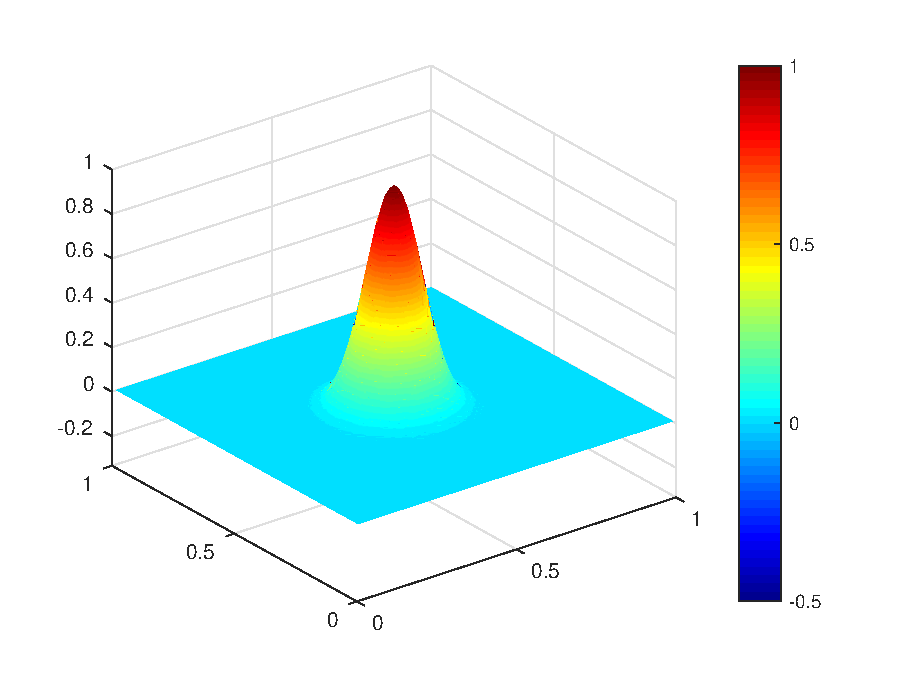
\includegraphics[height=4cm]{waves_t0.eps}
\includegraphics[height=4cm]{waves_t05.eps}
\includegraphics[height=4cm]{waves_t1.eps}
\end{center}
\caption{Solutions numériques pour l'équation des ondes \eqref{eq:ondes_2D} aux temps $t=0$, $t=0.5$ et $t=1$, $N=64$, $\Delta t=\Delta t_{\infty} \approx 5.7616\times10^{-4}$. La solution est obtenue par l'algorithme \ref{alg:RK4_ondes2d} avec un filtrage d'ordre 10 pour la condition initiale \eqref{eq:waves_test1}.}
\label{fig:waves_solution}
\end{figure}
\begin{figure}[htbp]
\begin{center}
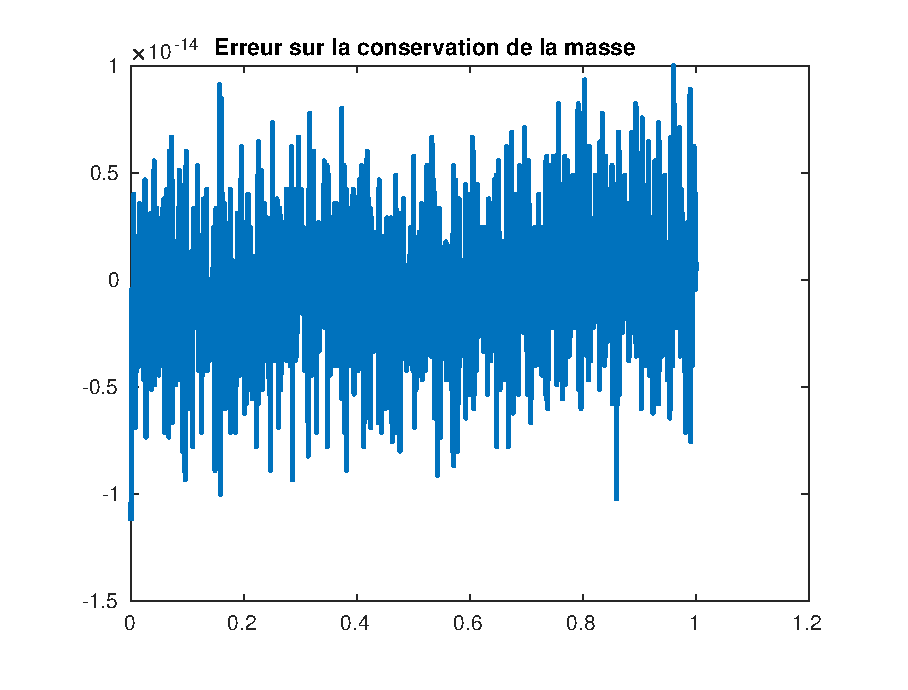
\includegraphics[height=5cm]{waves_mass.eps}
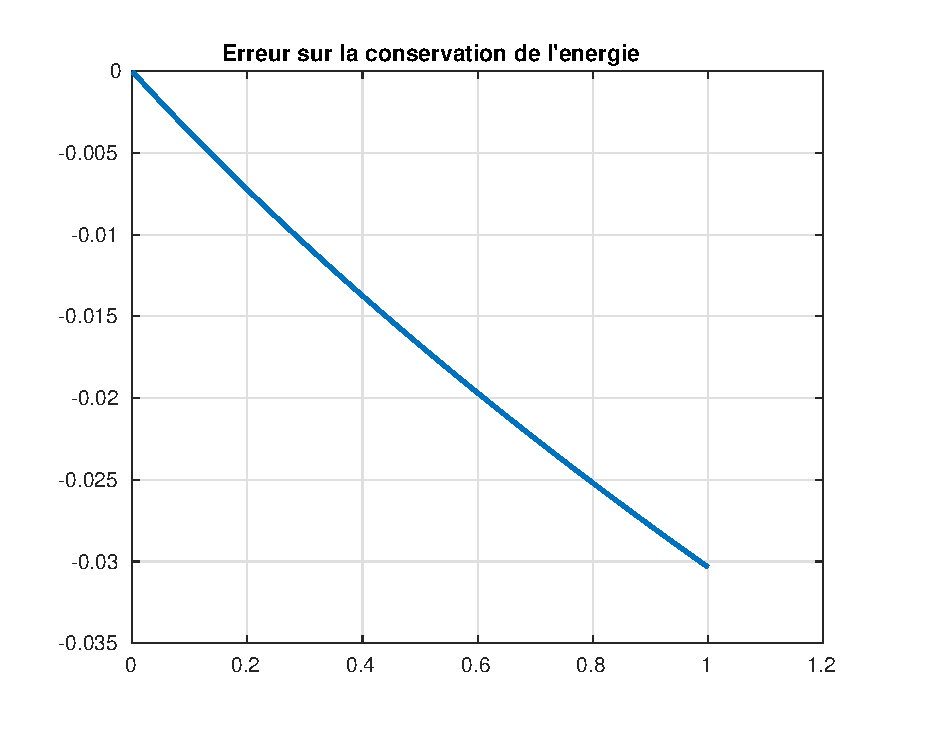
\includegraphics[height=5cm]{waves_energy.eps}
\end{center}
\caption{Erreur relative lors de la résolution de \eqref{eq:ondes_2D} sur la conservation de la masse et de l'énergie obtenue pour le test \eqref{eq:waves_test1} en utilisant l'algorithme \ref{alg:RK4_ondes2d} avec un filtrage d'ordre 10, $N=64$, $\Delta t=\Delta t_{\infty} \approx 5.7616\times10^{-4}$.}
\label{fig:waves_conservation}
\end{figure}
L'algorithme \ref{alg:RK4_ondes2d} est stable pour le pas de temps
\begin{equation}
\Delta t \leq \Delta t_{\infty} = \dfrac{2 \sqrt{2}}{\sqrt{\dfrac{6 g H}{h^2} + f^2}},
\end{equation}
avec ou sans filtrage. La table \ref{tab:dt_critique_waves} montre la recherche du pas de temps maximal pour lequel l'algorithme \ref{alg:RK4_ondes2d} est stable pour donnée initiale \eqref{eq:waves_test1}. Le pas de temps final est $T=2$ et le paramètre de la grille est $N=32$. On constate que plus l'ordre du filtre est bas, plus il est possible de choisir un pas de temps grand. Dans la table \ref{tab:conservation_waves}, on observe que choisir un filtrage d'ordre trop bas peut avoir des répercussions sur la conservation de l'énergie (la masse est toujours exactement conservée). Un filtrage d'ordre 2 ne permet pas de conserver l'énergie et un filtrage d'ordre 4 donne une dégradation de l'ordre de convergence. En revanche les filtrages d'ordre 8 et 10 donnent des résultats semblables.

\begin{table}[htbp]
\begin{center}
\begin{tabular}{|c||c|c|}
\hline
\textbf{Ordre du filtre : } $\mathbf{\mathcal{F}}$ : $\mathbf{2J}$  & \textbf{Instable pour} $\mathbf{\Delta t =}$ & \textbf{Stable pour} $\mathbf{\Delta t =}$ \\
\hline
\hline
Pas de filtrage & $1.16(-3)$ & $\Delta t_{\infty} \approx 1.15(-3)$\\
10 & $1.23(-3)$ & $1.22(-3)$ \\
8 & $1.26(-3)$ & $1.25(-3)$ \\
6 & $1.32(-3)$ & $1.31(-3)$ \\
4 & $1.41(-3)$ & $1.4(-3)$ \\
2 & $1.66(-3)$ & $1.65(-3)$ \\
\hline
\end{tabular}
\end{center}
\caption{Equation \eqref{eq:ondes_2D}. Stabilité de l'algorithme \ref{alg:RK4_ondes2d} pour $T=2$ pour la donnée initiale \eqref{eq:waves_test1}, $N=32$.}
\label{tab:dt_critique_waves}
\end{table} 


\begin{table}[htbp]
\begin{center}
\begin{tabular}{|c||c|c|c|c|c|c|c|}
\hline
$\mathbf{N \text{ et } \Delta t _{\infty}}$ & \textbf{Pas de filtre} & \textbf{Ordre 10} & \textbf{Ordre 8} & \textbf{Ordre 6} & \textbf{Ordre 4} & \textbf{Ordre 2}\\
\hline
$32\text{ et }1.1523(-3)$ & $2.5340(-1)$ & $2.5367(-1)$ & $2.5709(-1)$ & $3.0173(-1)$ & $6.2132(-1)$ & $9.3717(-1)$ \\
\hline
$64\text{ et }5.7616(-4)$ & $3.0328(-2)$ & $3.0347(-2)$ & $3.0802(-2)$ & $4.3763(-2)$ & $3.0419(-1)$ & $9.3712(-1)$ \\
\hline
$128\text{ et }2.8808(-4)$& $1.2226(-3)$ & $1.2227(-3)$ & $1.2301(-3)$ & $1.9323(-3)$ & $7.7084(-2)$ & $9.3398(-1)$ \\
\hline
\hline
\textbf{Ordre :} & $3.85$ & $3.85$ & $3.85$ & $3.64$ & $1.51$ & $2.46(-3)$ \\
\hline 
\end{tabular}
\end{center}
\caption{Equation \eqref{eq:ondes_2D}. Convergence de la conservation de l'énergie pour l'algorithme \ref{alg:RK4_ondes2d} et la donnée initiale \eqref{eq:waves_test1}. On représente l'erreur relative maximale pour $t<1$. Un filtre d'ordre $2$ ne permet pas de conserver l'énergie. Avec un filtre d'ordre $4$ l'énergie est conservée à un ordre bas. Pour un filtre d'ordre plus élevé, la convergence se fait à un ordre plus élevé.}
\label{tab:conservation_waves}
\end{table} 






























\section{Equation de Burgers}

Dans cette section, on considère l'équation de Burgers en contexte périodique \cite{Burgers1948, Witham1974} :
\begin{equation}
\left\lbrace
\begin{array}{rcl}
\dfrac{\partial u}{\partial t} + 2 \pi \dfrac{\partial}{\partial x} \left( \dfrac{u^2}{2} \right) & = & 0 \\
u(t=0,x) & = & u_0(x)
\end{array}
\right. \text{ pour } x \in [0, 2\pi] \text{ et } t \geq 0.
\label{eq:Burgers_1d}
\end{equation}
Une donnée initiale $u_0$ périodique non constante, conduit nécessairement à l'apparition d'un choc en temps fini. Le but de cette étude est double
\begin{enumerate}
\item Nous utilisons le schéma hermitien centré $\delta_{4,x}^H$ donné par la définition \ref{def:herder}  avec le filtre linéaire $\mathcal{F}_{2J,x}$ \eqref{eq:ftr} pour l'équation \eqref{eq:Burgers_1d}. Il est bien connu qu'un tel schéma est insuffisant pour obtenir une solution numérique sans oscillations. Le but est ici d'observer précisément comment les filtres linéaires $\mathcal{F}_{2J,x}$ agissent à l'approche du choc. Nous renvoyons à \cite{Yee1989, Cook2005} pour des études plus avancées utilisant des opérateurs de type filtre non linéaire, ou des opérateurs d'hyperdiffusion.

\item L'équation de Burgers périodique a été utilisée par \cite{BenArtzi2009} pour construire une famille particulière d'équations aux dérivées partielles sur la sphère conduisant à des chocs. Une telle solution sera analycée numériquement dans le chapitre \ref{chap:advection}.
\end{enumerate}

Nous supposerons que la donnée initiale $u_0$ est périodique et est telle que $u_0 \in \mathcal{C}^1([0,2 \pi])$ et $u_0' \in L^{\infty}([0,2 \pi])$.

\begin{theoreme}
L'équation \eqref{eq:Burgers_1d} admet une unique solution $u$ telle que
\begin{itemize}
\item $u \in \mathcal{C}^1(\mathbb{R}^+ \times [0, 2 \pi])$ si $u_0'(x) \geq 0$ pour tout $x \in [0,2 \pi]$,

\item $u \in \mathcal{C}^1\left(\left[0, -\frac{1}{\inf_{x \in [0,2\pi]} (2 \pi u_0'(x))}\right] \times [0, 2 \pi]\right)$, sinon.
\end{itemize}
De plus, cette solution $u$ vérifie pour $x \in [0, 2 \pi]$
\begin{equation}
u(t,2 \pi u_0(x)t + x)=u_0(x).
\end{equation}
\end{theoreme}

\begin{proof}
On étudie l'équation \eqref{eq:Burgers_1d} par la méthode des caractéristiques. Dans un premier temps, on suppose que $u \in \mathcal{C}^1$ solution de \eqref{eq:Burgers_1d} existe. Soit $X : \mathbb{R}^+ \mapsto \mathbb{R}$ une courbe telle que
\begin{equation}
\left\lbrace
\begin{array}{rcl}
X'(t) & = & 2 \pi u (t, X(t)) \\
X(0) & = & x
\end{array}
\right. .
\label{eq:systeme_eq_caract}
\end{equation}
D'après le théorème de Cauchy-Lipschitz, comme $X \mapsto 2 \pi u (t, X)$ est $\mathcal{C}^1$, il existe une solution maximale à \eqref{eq:systeme_eq_caract}.

Dès lors, on a que $g : t \mapsto u(t,X(t))$ est constante, en effet
\begin{align*}
g'(t) & = \dfrac{\partial u}{\partial t}(t,X(t)) + X'(t) \dfrac{\partial u}{\partial x} (t,X(t)) \\
	& = \dfrac{\partial u}{\partial t}(t,X(t)) + 2 \pi u (t, X(t)) \dfrac{\partial u}{\partial x} (t,X(t)) \\
	& = \dfrac{\partial u}{\partial t}(t,X(t)) + 2 \pi  \dfrac{\partial }{\partial x} \left( \dfrac{u(t,X(t))^2}{2} \right) \\
	& = 0.
\end{align*}
Comme $t \mapsto u(t,X(t))$ est constante, on a en particulier $2 \pi u (t, X(t)) = u_0(x)$ donc $X$ est en fait solution de 
\begin{equation}
\left\lbrace
\begin{array}{rcl}
X'(t) & = & 2 \pi u_0(x) \\
X(0) & = & x
\end{array}
\right. .
\label{eq:systeme_eq_caract2}
\end{equation}
donc $X$ est donné par
\begin{equation}
X(t) = 2 \pi u_0(x) t + x.
\end{equation}
$u$ est constante le long de $X$ donc $u$ vérifie
\begin{equation}
u(t,2 \pi u_0(x)t + x)=u_0(x).
\end{equation}

Cependant, ce résultat n'est vrai que si \eqref{eq:Burgers_1d} admet une solution de classe $\mathcal{C}^1$.
Posons $X_t(x) = 2 \pi u_0(x)t + x$, donc
\begin{equation}
X_t'(x) = 2 \pi u_0'(x) t + 1.
\end{equation}
Comme $u_0$ est régulière sur un compact, il existe $m \in \mathbb{R}$ tel que
\begin{equation}
m = \inf_{x \in [0, 2 \pi]} \left( 2 \pi u_0'(x) \right)
\end{equation}
deux cas de figures se présentent alors
\begin{itemize}
\item $m \geq 0$, alors pour tout $x \in [0, 2 \pi]$ et $t \geq 0$, on a $X'_t(x) > X'_0(x) = 1$ et $X_t$ est une bijection de $[0, 2 \pi]$ dans $X_t([0, 2 \pi]) = \mathbb{R}$,

\item soit $m < 0$ alors en posant $T = -1/m$, on a pour tout $t \in [0, T[$
\begin{equation}
X'_t(x) \geq m(t-T) > 0
\end{equation}
alors $X_t$ est i,e bijection de $[0, 2 \pi]$ dans $\mathbb{R}$.
\end{itemize}

Si $u \in \mathcal{C}^1$ est solution \eqref{eq:Burgers_1d} telle que $X_t$ est i,e bijection alors
\begin{equation}
u(t,x) = u_0(X_t^{-1}(x))
\end{equation}
et $X_t$ est une bijection si $m \geq 0$ ou si $m<0$ et $t \in [0, T[$.

Vérifions que $u : (t,x) \mapsto u(t,x) = u_0(X_t^{-1}(x))$ est bien solution et de classe $\mathcal{C}^1$ (pour $t$ tel que $X_t^{-1}$ est bien défini).

$X_t$ est de class $\mathcal{C}^1$, si $X_t'(x)>0$ pour tout $x \in [0, \pi]$ alors $X_t$ est inversible, $X_t^{-1}$ est $\mathcal{C}^1$. Pour tout $x \in [0,2 \pi]$, on a
\begin{equation}
(X_t^{-1})'(x) = \dfrac{1}{X_t'(X_t^{-1}(x))},
\end{equation}
donc en dérivant $u$ par rapport à $x$, on obtient
\begin{align*}
\dfrac{\partial u}{\partial x}(t,x) & = \dfrac{u_0'(X_t^{-1}(x))}{X_t'(X_t^{-1}(x))} \\
	& = \dfrac{u_0'(X_t^{-1}(x))}{1 + 2 \pi u_0'(X_t^{-1}(x))},
\end{align*}
d'où la formule suivante 
\begin{equation}
\dfrac{\partial u}{\partial x}(t,x)=\dfrac{u_0'(X_t^{-1}(x))}{1 + 2 \pi u_0'(X_t^{-1}(x))}
\label{eq:der_u_burgers_proof}
\end{equation}
Or, on sait que 
\begin{align*}
X_t(x) & = x + 2 \pi t u_0(x) \\
	& = x + 2 \pi t u(t,2 \pi u_0(x) t + x)\\
	& = x + 2 \pi t u(t,X_t(x)).
\end{align*}
Donc $x = X_t(x) - 2 \pi t u(t,X_t(x))$, d'où
\begin{equation}
X_t^{-1}(x) = x - 2 \pi t u(t,x).
\end{equation}
De là, on peut déduire la dérivée de $X_t^{-1}$ en temps :
\begin{equation}
\dfrac{\partial X_t^{-1}}{\partial t}(x) = - 2 \pi u(t,x) - 2 \pi t \dfrac{\partial u}{\partial t}(t,x).
\end{equation}
On en déduit :
\begin{align*}
\dfrac{\partial u}{\partial t}(tx,) & = \dfrac{\partial}{\partial t} u_0(X_t^{-1}(x)) \\
	& = \dfrac{\partial X_t^{-1}}{\partial t}(x) u_0'(X_t^{-1}(x)) \\
	& = (- 2 \pi u(t,x) - 2 \pi t \dfrac{\partial u}{\partial t}(t,x)) u_0'(X_t^{-1}(x)).
\end{align*}
Il découle :
\begin{equation}
\dfrac{\partial u}{\partial t}(t,x) \underbrace{(1 + 2 \pi t u_0'(X_t^{-1}(x)))}_{>0 \text{ lorsque } X_t^{-1} \text{est défini.}} = - 2 \pi u(t,x) u_0'(X_t^{-1}(x)).
\end{equation}
Donc, par division, on a
\begin{align*}
\dfrac{\partial u}{\partial t}(t,x) & = - \dfrac{2 \pi u(t,x) u_0'(X_t^{-1}(x))}{1 + 2 \pi t u_0'(X_t^{-1}(x))} \\
	& = - 2 \pi u(t,x) \dfrac{u_0'(X_t^{-1}(x))}{1 + 2 \pi u_0'(X_t^{-1}(x))} \\
	& = - 2 \pi u(t,x) \dfrac{\partial u}{\partial x}(t,x) \text{ d'après \eqref{eq:der_u_burgers_proof}.} \\
	& = - 2 \pi \dfrac{\partial}{\partial x}\left( \dfrac{u(t,x)^2}{2} \right)
\end{align*}
donc $u$ est bien solution de \eqref{eq:Burgers_1d} et par composition c'est une fonction $\mathcal{C}^1$ sur les intervalles souhaités.
\end{proof}

\begin{remarque}
\begin{itemize}
\item Pour que $u$ solution de \eqref{eq:Burgers_1d} soient une solution $\mathcal{C}^1$ en tout temps $t \geq 0$, il faut que $u_0$ soit $\mathcal{C}^1$ et de dérivée positive ou nulle. Compte tenue de la périodicité, cela implique $u_0$ constante.

\item Si $u_0$ est définie pour $x \in [0, 2 \pi]$ par 
\begin{equation}
u_0(x) = \sin (x)
\label{eq:burgers_expemple2}
\end{equation}
l'équation \eqref{eq:Burgers_1d} admet une unique solution de classe $\mathcal{C}^1$ pour $t \in [1, 1/(2\pi)]$. Au delà de cet intervalle, des chocs peuvent apparaître, la solution de \eqref{eq:Burgers_1d} n'est plus régulière.
\end{itemize}
\end{remarque}


Les chocs rendent les solution difficiles à représenter par des schémas aux différences finies car des phénomènes haute-fréquence important sont présents. Nous souhaitons, dans cette partie, observer les performances d'un schéma numérique donné par l'algorithme \ref{alg:RK4_burgers1d} pour l'équation \eqref{eq:Burgers_1d} où $\mathfrak{u}^n$ est une approximation de $u^*(t^n)$.

\begin{center}
\begin{minipage}[H]{12cm}
  \begin{algorithm}[H]
    \caption{: RK4}\label{alg:RK4_burgers1d}
    \begin{algorithmic}[1]
    \State $\mathfrak{u}^0 = u_0^*$ connu,
    \For{$n=0,1, \ldots$}
             \State  $K^{(1)} = - \pi \delta_{4,x}^H \left(\left( \mathfrak{u}^n \right)^2\right)$,
             \State  $K^{(2)} = - \pi \delta_{4,x}^H \left(\left( \mathfrak{u}^n + \dfrac{\Delta t}{2} K^{(1)}\right)^2\right)$,
             \State  $K^{(3)} = - \pi \delta_{4,x}^H \left(\left( \mathfrak{u}^n + \dfrac{\Delta t}{2} K^{(2)}\right)^2\right)$,
             \State  $K^{(4)} = - \pi \delta_{4,x}^H \left(\left( \mathfrak{u}^n + \Delta t K^{(3)}\right)^2\right)$,  
             \State  $\mathfrak{u}^{n+1} = \mathcal{F}_{2J,x}\left( \mathfrak{u}^n  + \dfrac{\Delta t}{6} \left( K^{(1)} + 2 K^{(2)} + 2 K^{(3)} + K^{(4)} \right) \right)$.
            \EndFor
    \end{algorithmic}
    \end{algorithm}
\end{minipage}
\end{center}

On peut directement démontrer la proposition suivante :
\begin{proposition}
Pour tout $n \in \mathbb{N}$, si $\mathfrak{u}^n$ est calculée par l'algorithme \ref{alg:RK4_burgers1d} alors
\begin{equation}
(\mathfrak{u}^{n+1}, \mathfrak{1})_{h,\per} = (\mathfrak{u}^n, \mathfrak{1})_{h,\per}.
\end{equation}
où $\mathfrak{1}$ est la fonction de grille constante égale à 1.
\end{proposition}

Les résultats sont pour $u_0$ donné par \eqref{eq:burgers_expemple2} et pour l'algorithme \ref{alg:RK4_burgers1d} sans filtrage dans la figure \ref{fig:comp_burgers}. Des oscillations parasites apparaissent et rendent le calcul très instable. Le schéma numérique ne donne plus de résultats au temps $t=0.5$.

\begin{figure}[htbp]
\begin{center}
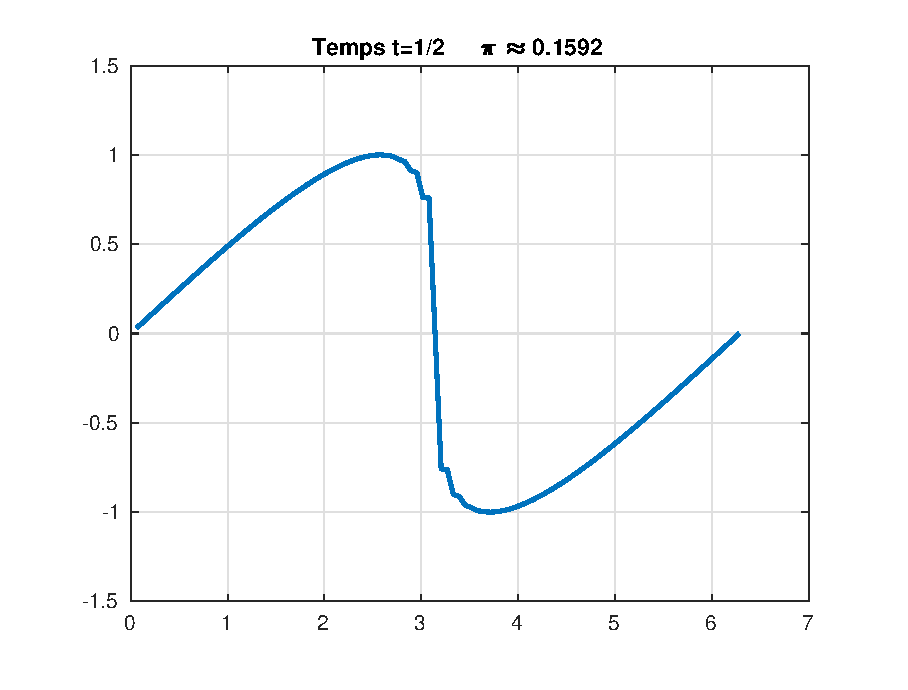
\includegraphics[height=5cm]{burgers_t1.eps}
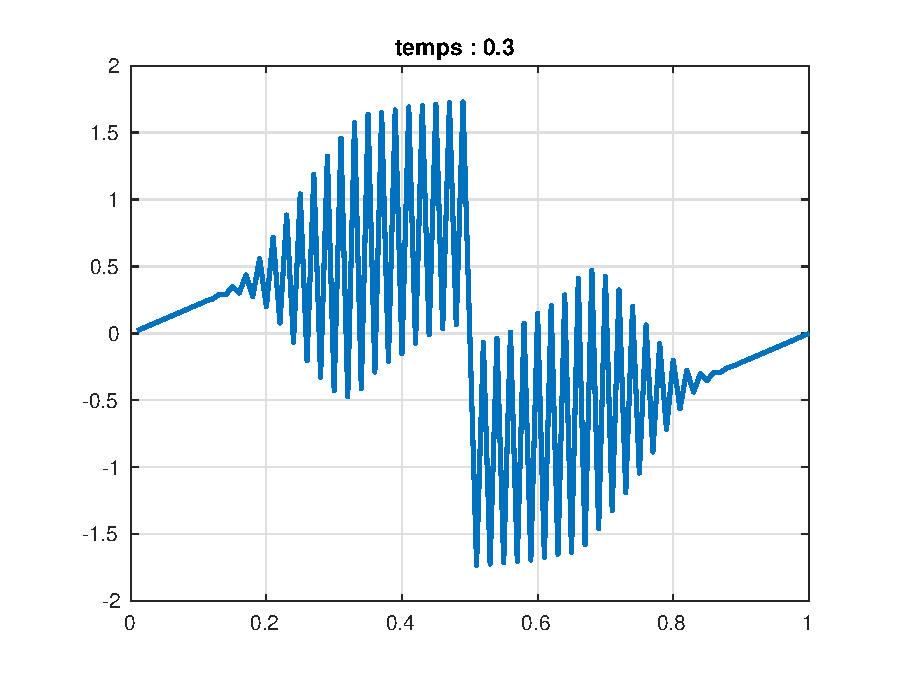
\includegraphics[height=5cm]{burgers_t2.eps}
\end{center}
\caption{Comparaison de la solution numériques obtenue par l'algorithme \ref{alg:RK4_burgers1d} sans opérateur de filtrage (c'est à dire $\mathcal{F}_{2J,x} = \Id$)à différents temps pour la résolution de l'équation \eqref{eq:Burgers_1d}. On choisit ici $N=100$ et $\Delta t = 10^{-3}$.}
\label{fig:comp_burgers}
\end{figure}

On compare la solution obtenue à l'aide de l'algorithme \ref{alg:RK4_burgers1d} en utilisant différents ordres pour l'opérateur de filtrage. Les résultats sont donnés en figure \ref{fig:comp_burgers_ftr}.

\begin{figure}[htbp]
\begin{center}
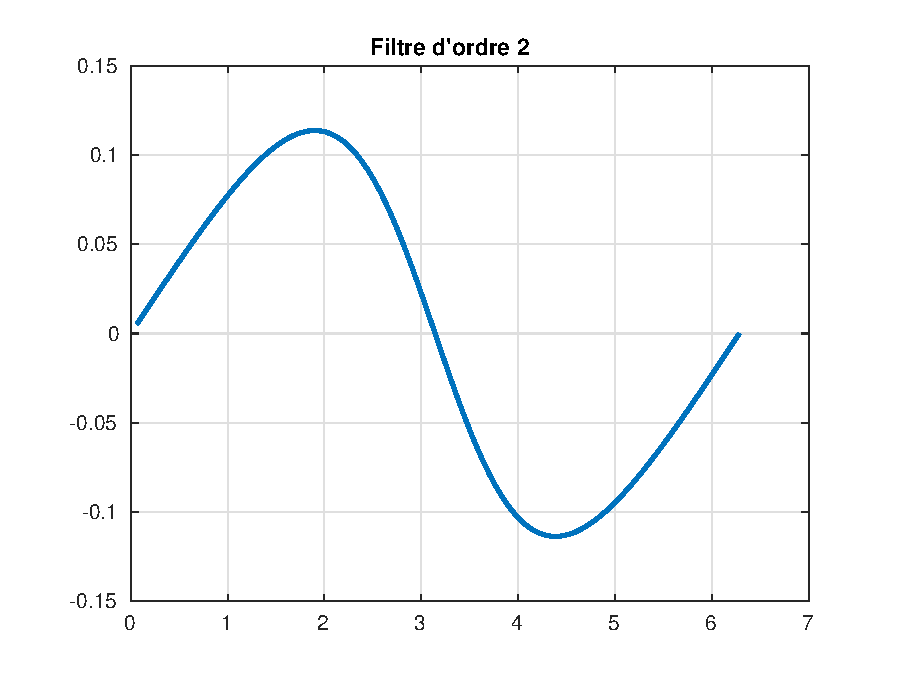
\includegraphics[height=5cm]{burgers_ftr2.eps}
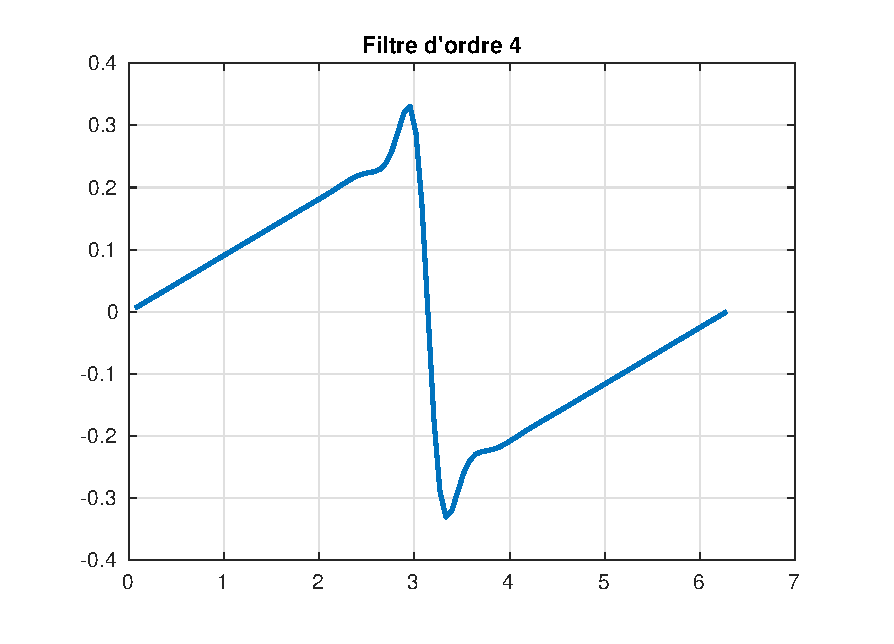
\includegraphics[height=5cm]{burgers_ftr4.eps}\\
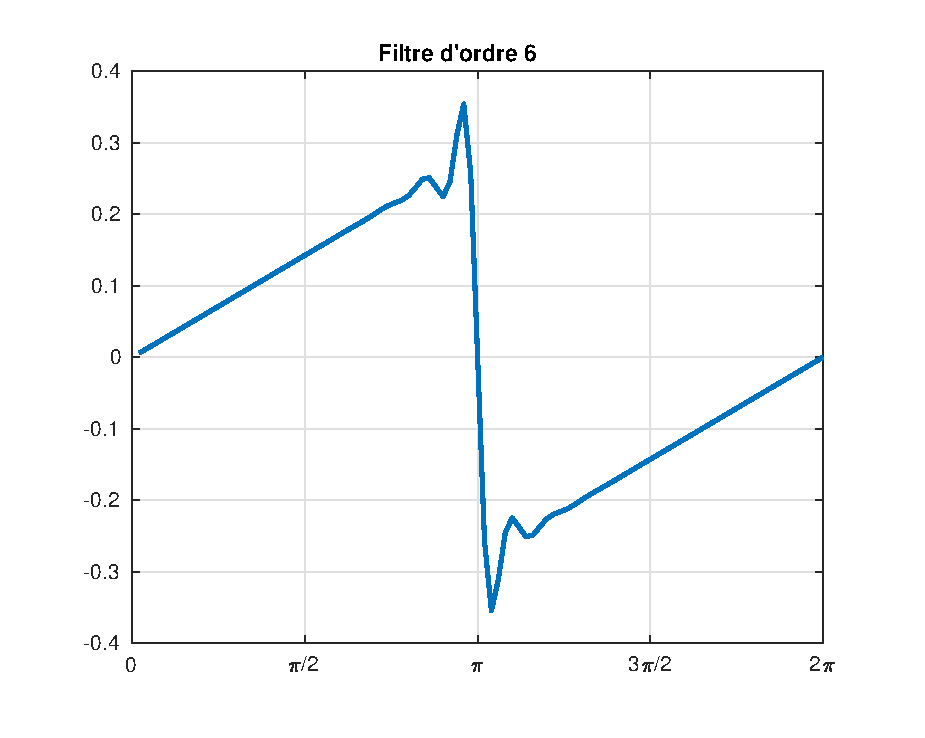
\includegraphics[height=5cm]{burgers_ftr6.eps}
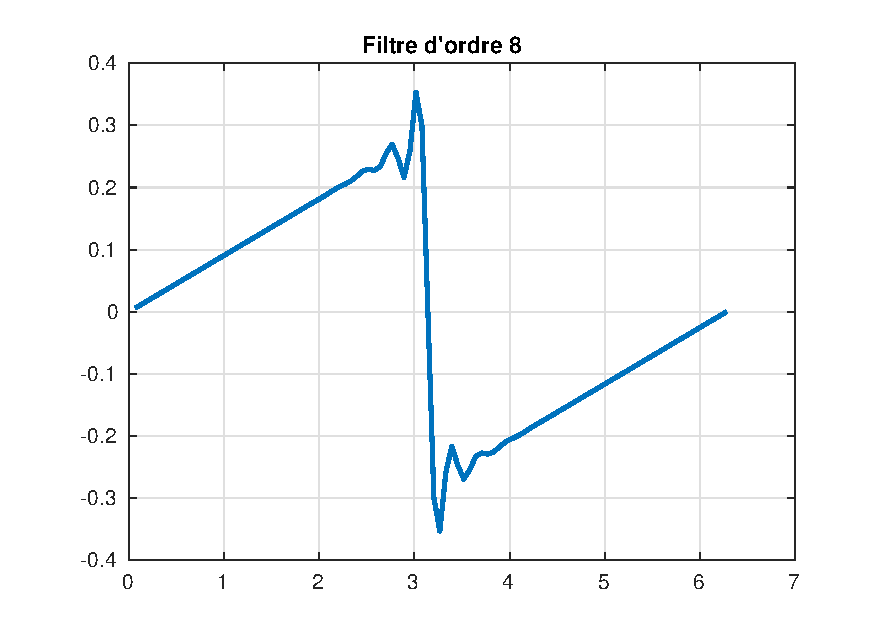
\includegraphics[height=5cm]{burgers_ftr8.eps}\\
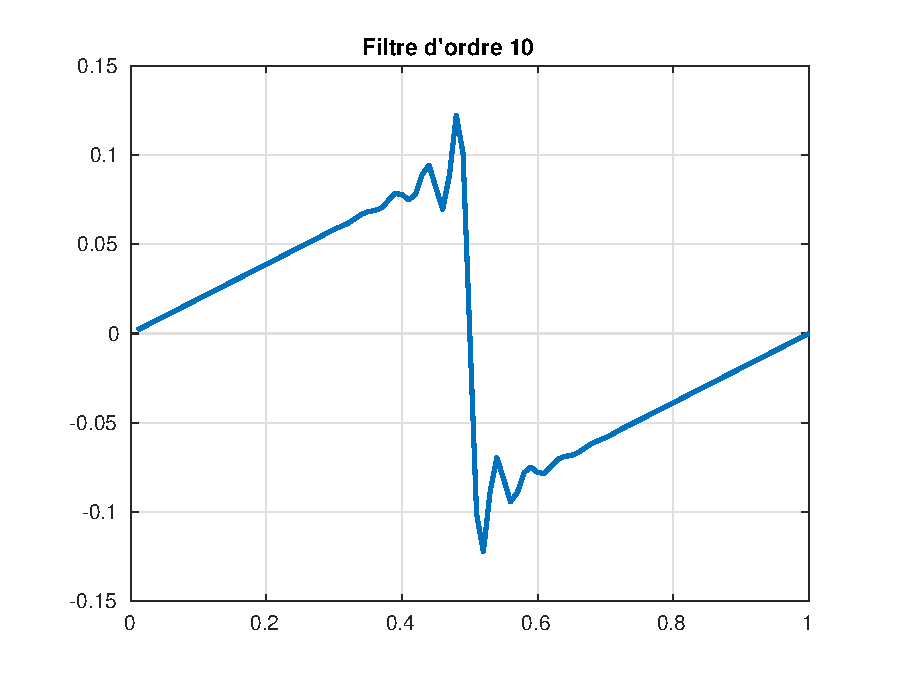
\includegraphics[height=5cm]{burgers_ftr10.eps}
\end{center}
\caption{Comparaison de différentes solution numériques de \eqref{eq:Burgers_1d} obtenue par l'algorithme \ref{alg:RK4_burgers1d} au temps $t=10/(2 \pi) \approx 1.5920$ avec différents filtres. $N=100$ et $\Delta t = 10^{-3}$.}
\label{fig:comp_burgers_ftr}
\end{figure}

Le filtrage d'ordre 2 est trop dissipatif. Les filtrages d'ordres plus élevés représentent mieux le choc et permettent au schéma de rester stable jusqu'à $t=10/(2 \pi)$ au minimum.

































